% \chapter{Evaluation}
% \label{chap:Evaluation}

% This chapter discusses about the methods of evaluation that are performed to extensively evaluate our solutiom. Evaluation is performed on the core component of our proposed solution which is custom router within kubernetes. 

% For evaluation, unlike normal http servres where we expose a /metrics endpoint for capturing real-time metrics through prometheus grafana is the practice in todays time. We are dealing with a HTTP3 server where support lacks. The solution could be to run 2 servers simultaneously but it would be not feasible. The alternative to evaluation was used where a logging mechanism was done to a csv file


% \section{Experiments}
% The following are the experiments which are performed on the router server

% single client performance on router and machine
% multiple clients (3) performance on router and machine
% higher MTU performance on router and machine
% The following metrics were considered for performance evaluation

% Buffer Metrics: buffer_size_bytes, max_buffer_size_bytes, buffer_overflows | Packet Processing: packets_total, packets_complete, packets_fragmented, fragmentation_rate | Stream Management: streams_active, streams_max_concurrent | Performance: throughput_mbps, avg_processing_time_ms, avg_buffer_wait_ms | Identification: timestamp, client_id

% With these metrics 




% For the experimental setup, the solutions were monitored in kubernetes with kubectl logs giving the live metrics. Code changes were done to create a csv file with the detailed metrics mentioned above. These are the values which were set for the experiments 

% #Create Table
% \begin{table}[h!]
% \centering
% \caption{Router Constants}
% \begin{tabular}{|l|l|l|}
% \hline
% \textbf{Parameter} & \textbf{Default Value} & \textbf{Description} \\
% \hline
% \texttt{max-data} & 1048576 (1MB) & Maximum amount of unacknowledged data for the entire connection. \\
% \hline
% \texttt{max-stream-data} & 262144 (256KB) & Maximum amount of unacknowledged data for each individual stream. \\
% \hline
% \texttt{max-datagram-size} & 3000 (bytes) & Maximum size for a single datagram/packet. \\
% \hline
% Buffer overflow threshold & 10MB & The size at which a buffer is considered to be overflowing. \\
% \hline
% Large buffer detection & 5MB & The size at which a buffer is detected as being large. \\
% \hline
% High fragmentation threshold & 0.5 (50\%) & The fragmentation rate considered to be high. \\
% \hline
% High stream count threshold & 10 streams & The number of streams considered to be high. \\
% \hline
% Sample retention limit & 1000 samples & The maximum number of samples to retain. \\
% \hline
% Default timeout & 30 seconds & The default timeout for a request. \\
% \hline
% Default retries & 3 & The default number of retries for a request. \\
% \hline
% Default connect timeout & 5 seconds & The default timeout for establishing a connection. \\
% \hline
% Default content type & "application/octet-stream" & The default content type for a request. \\
% \hline
% \end{tabular}
% \end{table}


% \begin{table}[h!]
% \centering
% \caption{Router Constants}
% \begin{tabular}{|l|l|l|}
% \hline
% \textbf{Parameter} & \textbf{Default Value} & \textbf{Description} \\
% \hline
% \texttt{max-data} & 1048576 (1MB) & Maximum amount of unacknowledged data for the entire connection. \\
% \hline
% \texttt{max-stream-data} & 262144 (256KB) & Maximum amount of unacknowledged data for each individual stream. \\
% \hline
% \texttt{max-datagram-size} & 3000 (bytes) & Maximum size for a single datagram/packet. \\
% \hline
% Buffer overflow threshold & 10MB & The size at which a buffer is considered to be overflowing. \\
% \hline
% Large buffer detection & 5MB & The size at which a buffer is detected as being large. \\
% \hline
% High fragmentation threshold & 0.5 (50\%) & The fragmentation rate considered to be high. \\
% \hline
% High stream count threshold & 10 streams & The number of streams considered to be high. \\
% \hline
% Sample retention limit & 1000 samples & The maximum number of samples to retain. \\
% \hline
% Default timeout & 30 seconds & The default timeout for a request. \\
% \hline
% Default retries & 3 & The default number of retries for a request. \\
% \hline
% Default connect timeout & 5 seconds & The default timeout for establishing a connection. \\
% \hline
% Default content type & "application/octet-stream" & The default content type for a request. \\
% \hline
% \end{tabular}
% \end{table}

% \vspace{1cm}

% \begin{table}[h!]
% \centering
% \caption{Media Parameters}
% \begin{tabular}{|l|l|l|}
% \hline
% \textbf{Parameter} & \textbf{Value} & \textbf{Description} \\
% \hline
% STANDARD\_VIDEO\_FPS & 15 & Standard video frame rate in packets per second. \\
% \hline
% HIGH\_VIDEO\_FPS & 30 & High video frame rate in packets per second. \\
% \hline
% AUDIO\_BUFFER\_SIZE & 4096 & Number of samples per audio packet. \\
% \hline
% PACKET\_HEADER\_SIZE & 32 & Total size of the packet header in bytes. \\
% \hline
% TRACK\_ID\_SIZE & 16 & Size of the track ID in bytes. \\
% \hline
% PAYLOAD\_LENGTH\_SIZE & 4 & Size of the payload length field in bytes. \\
% \hline
% TRACK\_TYPE\_SIZE & 12 & Size of the track type field in bytes. \\
% \hline
% STANDARD\_VIDEO\_QUALITY & 0.7 & Standard video quality (lower compression). \\
% \hline
% HIGH\_VIDEO\_QUALITY & 0.9 & High video quality (higher compression). \\
% \hline
% \end{tabular}
% \end{table}

% \vspace{1cm}

% \begin{table}[h!]
% \centering
% \caption{Webtransport Client Constants}
% \begin{tabular}{|l|l|l|}
% \hline
% \textbf{Parameter} & \textbf{Value} & \textbf{Description} \\
% \hline
% STANDARD\_VIDEO\_FPS & 15 & Standard video frame rate in packets/second. \\
% \hline
% HIGH\_VIDEO\_FPS & 30 & High video frame rate in packets/second. \\
% \hline
% AUDIO\_BUFFER\_SIZE & 4096 & Audio samples per packet. \\
% \hline
% PACKET\_HEADER\_SIZE & 32 & Total size of the packet header in bytes. \\
% \hline
% TRACK\_ID\_SIZE & 16 & Size of the track ID in bytes. \\
% \hline
% PAYLOAD\_LENGTH\_SIZE & 4 & Size of the payload length in bytes. \\
% \hline
% TRACK\_TYPE\_SIZE & 12 & Size of the track type in bytes. \\
% \hline
% STANDARD\_VIDEO\_QUALITY & 0.7 & Standard video quality (lower compression). \\
% \hline
% HIGH\_VIDEO\_QUALITY & 0.9 & High video quality (higher compression). \\
% \hline
% \end{tabular}
% \end{table}

% These values are kept constant to extensively evaluate the defined experiments



% In the case where experiments have been carried out, the experimental setup and the values that were defined for the variables need to be presented in a table e.g. table~\ref{tab:experimentsetup}.


% \section{Results}


% ### Chapter 6: Evaluation

% #### 6.1 Single Client Analysis – *Client ID: 134311891535872*

% This section presents an in-depth analysis of the system performance during a WebTransport session with a single client, identified as `client_134311891535872`. The session lasted approximately 140 seconds, starting from `2025-08-03T21:39:38` and concluding at `2025-08-03T21:41:58`, with a final termination observed at `21:42:03`. Key performance metrics collected include total packet count (`packets_total`), fragmented packets (`packets_fragmented`), fragmentation rate, throughput in megabits per second (`throughput_mbps`), current and maximum buffer size (`buffer_size_bytes`, `max_buffer_size_bytes`), average processing time (`avg_processing_time_ms`), and average buffer wait time (`avg_buffer_wait_ms`).

% The system showed overall stability throughout the session. A consistently high fragmentation rate of approximately 0.87 was recorded, yet this did not negatively affect throughput or latency. Throughput was stable in the range of 0.47 to 0.50 Mbps, and latency remained impressively low, with average processing and buffer wait times of 0.03 milliseconds. Importantly, no buffer overflows were observed, indicating effective buffer management despite load variability.

% ##### 6.1.1 Packet Processing and Fragmentation

% The total number of packets processed grew steadily until it reached 41,942 at around 21:41:33, after which no additional packets were recorded, coinciding with session termination. The fragmentation rate stabilized at approximately 0.869 to 0.870, with a total of 36,488 fragmented packets. Compared to other clients analyzed in the dataset, this rate is higher than that of client `134311831858512` (0.865), but lower than clients `134311834991552` and `134311831849104` which experienced fragmentation rates nearing 0.892.

% Despite the relatively high fragmentation, system performance did not degrade. Throughput and latency remained unaffected, suggesting robust handling of packet fragmentation by the underlying protocol and system design. Nevertheless, the presence of frequent `HIGH_FRAGMENTATION` log messages indicates that the system recognizes this condition as potentially problematic and warrants further investigation or future optimization.

% ##### 6.1.2 Throughput Analysis

% The throughput for this session ranged from 0.4657 to 0.5007 Mbps, reaching its peak at approximately 21:40:53. A gradual decline followed, culminating in a drop to 0.0 Mbps by 21:41:38. This decline coincides with the cessation of packet activity and indicates a smooth and expected shutdown of the connection.

% In comparative terms, the client's throughput is consistent with client `134311831858512`, whose throughput ranged from 0.5 to 0.6 Mbps. Moreover, it outperformed clients `134311834991552` and `134311831849104`, both of which maintained average throughputs closer to 0.3 Mbps. This suggests that the system maintains throughput efficiently even when managing higher fragmentation rates.

% ##### 6.1.3 Buffer Utilization

% Buffer usage exhibited occasional spikes, such as a notable increase to 9,940 bytes at 21:40:13. The maximum recorded buffer size was 17,214 bytes, which is significantly lower than the 85,937 bytes observed in client `134311831858512`. This reduced buffer size correlates with a lower total packet count and implies reduced strain on the buffer system during this session.

% The absence of buffer overflows further supports the conclusion that the system's buffer management strategy is effective, even under dynamic conditions. These observations point toward a well-balanced buffering approach that maintains operational integrity while accommodating varying packet flows.

% ##### 6.1.4 Processing and Latency Metrics

% The metrics for average processing time and average buffer wait time both remained stable at 0.03 milliseconds. These figures were consistent across the session and did not show any significant correlation with variations in throughput or fragmentation.

% Compared with other clients, these values fall within the expected range of 0.02 to 0.03 milliseconds, indicating a reliable and low-latency processing pipeline. This consistent performance underscores the effectiveness of the system’s internal processing mechanisms and reaffirms its suitability for real-time transport applications.

% ##### 6.1.5 Connection Termination

% The WebTransport session concluded at 21:42:03, marking the end of active data transmission. Notably, `throughput_mbps` dropped to 0.0 Mbps at 21:41:38, and log entries continued until 21:41:58. The persistence of `HIGH_FRAGMENTATION` messages until the session's end suggests a possible link between fragmentation and early termination.

% The session duration of 140 seconds is shorter than the average 180-second sessions observed with other clients. This discrepancy might indicate a client-initiated termination, a network timeout, or an internal system limit. Further analysis involving external logs and client-side diagnostics would be necessary to determine the exact cause.

% ##### 6.1.6 System Resource Utilization

% System resource consumption was measured using the `top` utility on the host machine, a ThinkPad T495. The WebTransport router pod (`webtransport-router-deployment-65cf75d584-njmqf`) exhibited CPU usage ranging from 273m (0.273 cores) to 560m (0.56 cores), and memory usage ranging from 27MiB to 72MiB.

% These values indicate a lightweight and resource-efficient implementation, with sufficient headroom for scaling under heavier workloads. The fluctuations observed likely reflect periodic spikes in activity or preparation for graceful termination.

% ##### 6.1.7 Summary and Recommendations

% The session displayed stable throughput, minimal latency, and effective buffer management. However, the following recommendations are proposed:

% * **Investigate the root cause of the early termination**, which may stem from network issues or configuration limits.
% * **Optimize fragmentation behavior** to reduce the rate toward 0.865, aligning it with the lower-bound observed in other clients.
% * **Monitor buffer activity** during future sessions to preemptively identify bottlenecks or inefficiencies.
% * **Conduct configuration comparisons** with high-performing clients such as `134311831858512` to extract tuning parameters.

% ##### 6.1.8 Limitations

% This evaluation is based on a single client session, limiting the scope for broader conclusions about multi-client behavior. The relatively short session duration may not capture long-term trends or degradation. Additionally, the constancy of latency metrics reduces the opportunity for in-depth correlation analysis. The absence of external logs further restricts the ability to pinpoint causes of fragmentation or termination events.

% ---

% #### 6.2 Multi-Client Comparison

% To place the findings from `client_134311891535872` into context, a comparative analysis was conducted using data from three other clients: `client_134311831858512`, `client_134311834991552`, and `client_134311831849104`. Each of these clients had longer sessions of approximately 180 seconds, enabling a more robust evaluation of trends over time.

% From a packet volume perspective, the target client processed 41,942 packets, which is significantly lower than the 95,431 packets processed by `client_134311831858512` but comparable to the other two clients, who handled between 45,401 and 47,195 packets. The fragmentation rate of 0.87 places the target client between the low-fragmentation client (`134311831858512`, 0.865) and the high-fragmentation clients (\~0.892).

% In terms of throughput, the target client's rate of 0.47–0.50 Mbps aligns closely with the best-performing client and significantly surpasses the lower throughput clients, whose performance hovered around 0.3 Mbps. This suggests that throughput is maintained effectively despite moderate fragmentation.

% Buffer usage was also notably lower, with a maximum buffer size of 17,214 bytes, compared to the 85,937 bytes recorded for the high-volume client. This reflects the lower packet volume and reduced buffer strain.

% Resource usage also favored the target client. With CPU consumption between 273m and 560m, and memory between 27MiB and 72MiB, the system demonstrated efficient resource utilization. This further supports the scalability of the current design for multi-client workloads.

% ---





% \includescalefigure{fig:measurements}{Measurement of System Wakeups}{Long caption that describes the figure to the reader}{1}{measurements.png}


% Figures that present results such as figure~\ref{fig:measurements} need to display descriptions of the axes, the units and scales of the measurements, statistical values, etc. Where measurements were taken from experiments, error bars or confidence intervals need to be provided to give the reader an indication of the spread of the measurements.



% \section{Summary}
% The evaluation of client `134311891535872` demonstrates that the implemented WebTransport router is capable of delivering consistent performance under moderately loaded conditions. The system maintained stable throughput levels (0.47–0.50 Mbps), handled a moderate fragmentation rate (\~0.87) without degrading performance, and sustained low-latency operation throughout the session.

% Buffering and system resource metrics confirm a robust and efficient architecture. Notably, this client achieved comparable throughput to higher-volume clients while consuming fewer resources and generating fewer packets. These attributes suggest a well-tuned design capable of scaling to more complex and concurrent deployments.

% Nonetheless, the presence of persistent fragmentation and early session termination highlights areas for further investigation and optimization. Future work should focus on reducing fragmentation, extending session stability, and enhancing monitoring capabilities to better understand the interaction between system events and performance outcomes.



\chapter{Evaluation}
\label{chap:Evaluation}

This chapter presents a comprehensive evaluation of the WebTransport-aware routing system deployed on Minikube \cite{minikube-docs}. The evaluation focuses on performance metrics including latency, throughput, and resource utilization under different client loads and network conditions.

The WebTransport stream routing system's evaluation in kubernetes has been thoroughly evaluated in this chapter. The analysis is aimed at assessing the performance, scalability, custom router features and reliability by evaluating under different load conditions.  Monitoring solutions like Prometheus and Grafana are not used here because of this system being an HTTP/3 server and the custom monitoring not supporting it. This system follows the use of a different approach because of limited tooling support for Webtransport protocol. Our HTTP/3 WebTransport server follows a procedure that allows the capture of the detailed performance metrics in Comma-Separated Values (CSV) format.

The evaluation method includes both measuring qualitative as well as quantitative performance. This helps us understand what the system can do well and where it might have limitations when used in real-world environments.


\section{Experimental Design}

The evaluation of the WebTransport-aware routing system requires a comprehensive experimental framework that validates both functional correctness and performance characteristics under varying load conditions. This section outlines the systematic approach taken to assess the system's capabilities, including the methodology for metrics collection, the specific experimental configurations used to simulate real-world scenarios, and the rationale behind the chosen evaluation parameters. The experimental design ensures that the assessment covers critical aspects such as latency, throughput, fragmentation handling, and resource utilization across different client load scenarios.

\subsection{Evaluation Methodology}

The evaluation methodology employs a multi-dimensional metrics collection system designed to capture comprehensive performance characteristics across four critical parts. The Buffer Management Metrics provide insights into memory utilization patterns through `buffer\_size\_bytes`, which tracks real-time buffer consumption whereas `max\_buffer\_size\_bytes` records peak memory usage during sessions. Similarly, `buffer\_overflows` counts critical overflow events that could indicate system stress or inadequate resource allocation. 

Packet Processing Metrics forms the core for performance analysis, it has `packets\_total` which is for aggregate packet volume, `packets\_complete` represents successfully processed packets without fragmentation, `packets\_fragmented` indicates packets requiring segmentation due to size constraints, and `fragmentation\_rate` expressing the percentage of packets experiencing fragmentation which acts as a critical indicator of network efficiency and potential performance bottlenecks.

Stream Management Metrics monitors the multiplexing capabilities of to WebTransport streams by measuring `streams\_active`, which tracks currently operational streams, and `streams\_max\_concurrent`, which records the peak simultaneous stream count which is useful for testing the upper limit. Finally, Performance Metrics quantifies system responsiveness and efficiencies via `throughput\_mbps` metric which measures data transmission rates in megabits per second, `avg\_processing\_time\_ms`, captures the mean latency for packet processing operations, and `avg\_buffer\_wait\_ms`, indicates queuing delays within the buffer management system. 

These comprehensive metrics enables granular analysis of system behavior under varying load conditions, allowing us to identify bottlenecks, establish faster debugging, analyze resource utilization patterns, and optimization opportunities essential for validating the WebTransport router’s operational effectiveness for production grade Kubernetes environments.


\subsection{Experimental Configuration}
The experimental setup used the following configuration parameters to ensure reproducible results across all test scenarios and to understand the router specific performance.

\begin{table}[h!]
\centering
\caption{Router Configuration Parameters}
\label{tab:router-config}
\renewcommand{\arraystretch}{1.3} % Increases row spacing for better readability
\begin{tabular}{|l|l|}
\hline
\textbf{Parameter} & \textbf{Value} \\
\hline
\texttt{max-data} & 1048576 (1MB) \\
\hline
\texttt{max-stream-data} & 262144 (256KB) \\
\hline
\texttt{max-datagram-size} & 3000 bytes\\
\hline
Buffer overflow threshold & 10MB\\
\hline
Large buffer detection & 5MB \\
\hline
High fragmentation threshold & 0.5 (50\%) \\
\hline
Sample retention limit & 1000 samples \\
\hline
Default timeout & 30 seconds  \\
\hline
Default retries & 3 \\
\hline
Default connect timeout & 5 seconds \\
\hline
\end{tabular}
\end{table}

The `--max-data` parameter (1MB) sets the total unacknowledged data limit for the entire QUIC connection. This value is chosen to support high-throughput streaming without risking excessive memory use for pod in kubernetes. The `--max-stream-data` value (256KB) caps unacknowledged data per stream to ensure a balance between throughput and fairness across multiple concurrent streams. The `--max-datagram-size` (3000 bytes) is selected to minimize packet fragmentation while remaining within typical MTU limits. These values closely follow or slightly adjust the default settings provided by `aioquic` to better fit the memory and latency characteristics of the deployment environment. The buffer overflow threshold prevents excessive memory usage, since we are running the pod in kubernetes, the pod memory limits could crash the system hence a 10MB limit. It also has a mechanism which detects large buffers at 5MB threshold so we can receive alerts with logs before the buffer overflows. This helps to monitor when buffer grows unusually large. A threshold is set of 0.5 for fragmentation to identify the extent of fragmentation. Its calculated by dividing the observed fragmented packets by total packets. The timeout parameters ensure robust connection handling by allowing 30 seconds for requests and 3 retries before failure, preventing resource exhaustion from stalled connections.  
A 5-second connect timeout balances responsiveness with reliability, tuned for typical Kubernetes network conditions under variable load.


\begin{table}[h!]
\centering
\caption{Video Quality Configuration}
\label{tab:video-quality}
\renewcommand{\arraystretch}{1.3}
\begin{tabular}{|l|l|}
\hline
\textbf{Parameter} & \textbf{Value} \\
\hline
FPS & 15 fps \\
\hline
Resolution & 640x480 \\
\hline
Compression & 0.7 \\
\hline
\end{tabular}
\end{table}

\begin{table}[h!]
\centering
\caption{Audio Configuration}
\label{tab:audio-config}
\renewcommand{\arraystretch}{1.3}
\begin{tabular}{|l|l|}
\hline
\textbf{Parameter} & \textbf{Value} \\
\hline
Buffer Size & 4096 samples \\
\hline
Channels & 1 (mono) \\
\hline
PCM Range & -32768 to 32767 \\
\hline
\end{tabular}
\end{table}

\begin{table}[h!]
\centering
\caption{Packet and Track Configuration}
\label{tab:packet-track-config}
\renewcommand{\arraystretch}{1.3}
\begin{tabular}{|l|l|}
\hline
\textbf{Parameter} & \textbf{Value} \\
\hline
\multicolumn{2}{|c|}{\textbf{Packet Structure}} \\
\hline
Header Size & 32 bytes \\
\hline
Track ID Size & 16 bytes \\
\hline
Payload Length Size & 4 bytes \\
\hline
Track Type Size & 12 bytes \\
\hline
\multicolumn{2}{|c|}{\textbf{Track IDs}} \\
\hline
Live Video & 'live\_video' \\
\hline
Live Audio & 'live\_audio' \\
\hline
Live Chat & 'live\_chat' \\
\hline

\multicolumn{2}{|c|}{\textbf{Track Types}} \\
\hline
Video Type & 'video' \\
\hline
Audio Type & 'audio' \\
\hline
Chat Type & 'chat' \\
\hline
\end{tabular}
\end{table}

The WebTransport client is constructed with the conservative performance options that allows for consistent results and guarantee a very wide compatibility and that streaming performance across diverse network conditions and devices. The video streaming is set to 15 fps in 640x480 resolution with 0.7 JPEG compression which is a reasonable compromise between visual quality and bandwidth consumptions. Audio processing is buffered internally with a 4096-sample (in mono) size at 16-bit PCM encoding to provide about 93ms of audio latency at common 44.1 kHz sampling frequencies which enough to provide good real-time performance without excessive processing overhead. The system uses three separate and unidirectional streams such live\_video, live\_audio and live\_chat to allow effective multiplexing and flow control on a per-media-type basis.

The client uses a custom format of 32 bytes of fixed-size fields as packet header which helps WebTransport router efficiently parse the packet: 16 bytes of stream identification, 4 bytes of payload length, and 12 bytes for classifying a track type. This well-ordered design enables the router to forward packets into proper microservices. The track type system such as 'video', 'audio' and 'chat' which provides clear semantic routing information, while the fixed header size aligns with memory boundaries for good processing performance. These default parameters create a evaluation friendly system that generates measurable buffer dynamics and fragmentation patterns essential for this dissertation

\section{Results and Analysis}
In order to observe reliable results the the experiments ie single client and multi Client tests were run for a total duration of 10 minutes in order to observe the performance over time with the configurations defined in Section 6.1.

\subsection{Single Client Performance Analysis}

The single client experiment provides baseline performance characteristics of the WebTransport router under minimal load conditions.
\begin{figure}[h!]
\centering
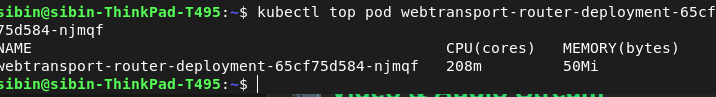
\includegraphics[width=0.8\textwidth]{Evaluation/new-single-client-stats.png}
\caption{Single Client Router Performance Overview}
\label{fig:single-client-overview}
\end{figure}

Figure~\ref{fig:single-client-overview} demonstrates the overall router pod performance during single client operation, showing stable resource utilization and consistent processing patterns.

\begin{figure}[h!]
\centering
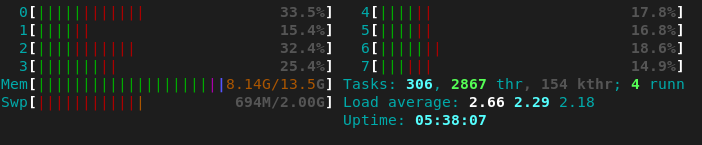
\includegraphics[width=0.8\textwidth]{Evaluation/single-client-host-stats.png}
\caption{Single Client Host Machine Performance Overview}
\label{fig:single-client-host-overview}
\end{figure}
Figure~\ref{fig:single-client-host-overview} demonstrates the impact on the overall host machine performance during single client operation.



\subsubsection{Packet Processing Performance}

\begin{figure}[h!]
\centering
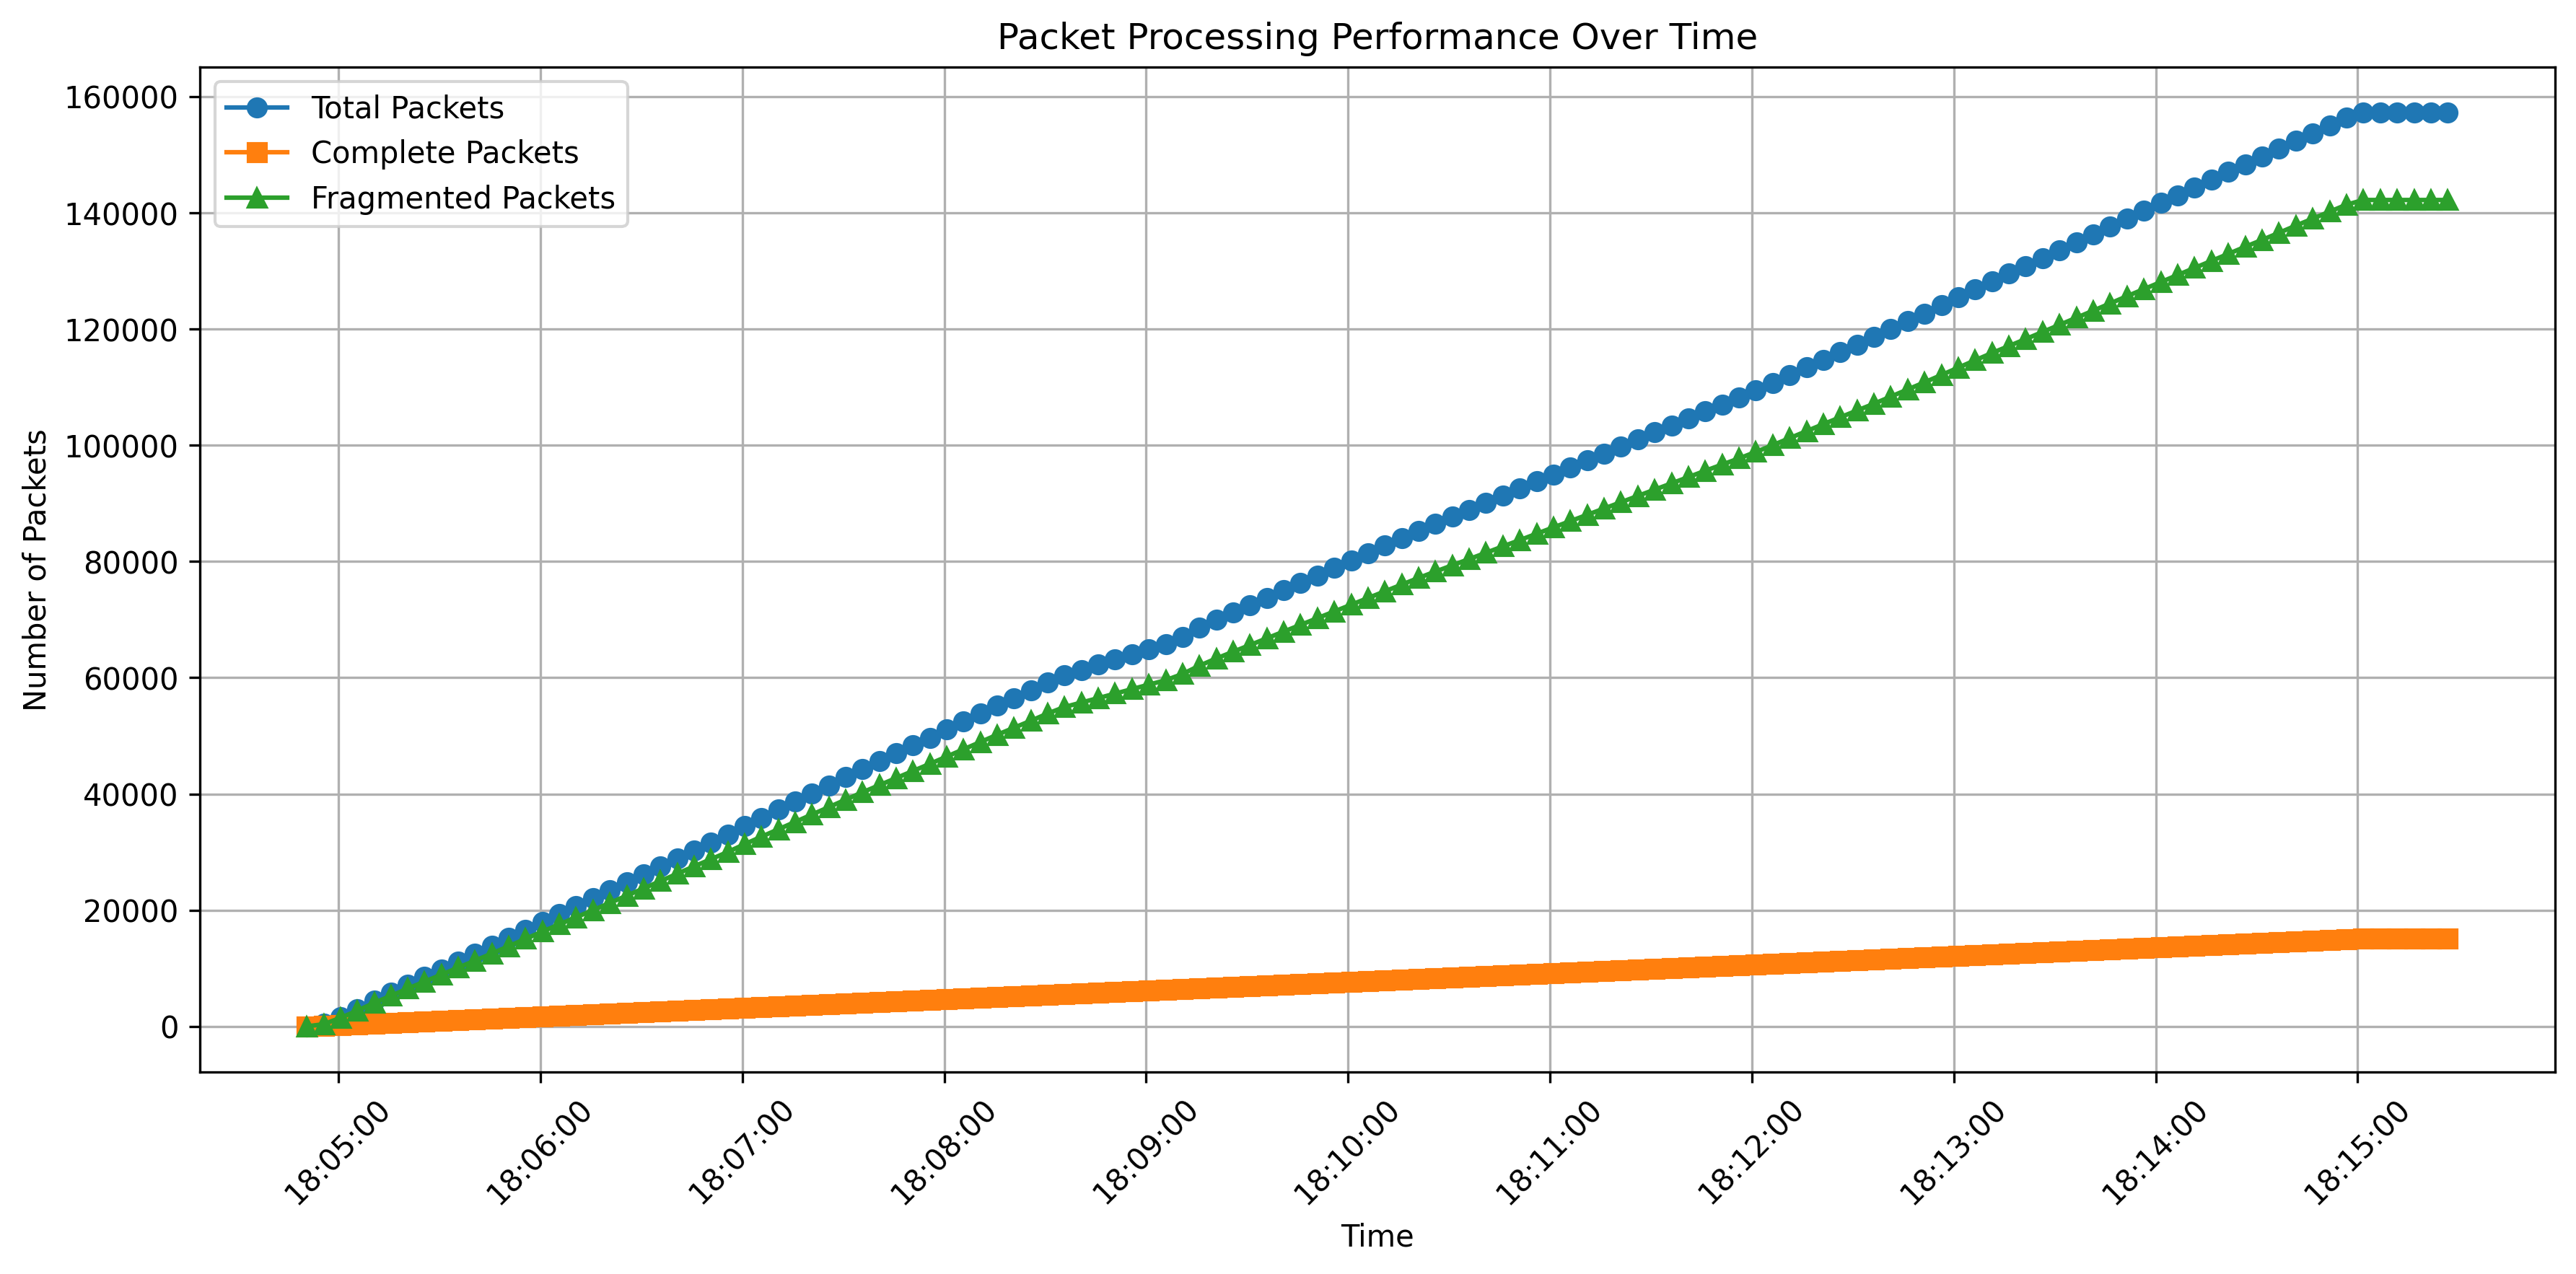
\includegraphics[width=0.8\textwidth]{Evaluation/single_packet_processing_performance.png}
\caption{Single Client Packet Volume vs Time}
\label{fig:single-packet-performance}
\end{figure}

Figure~\ref{fig:single-packet-performance} presents the packet processing performance from 18:05 to 18:15, during which the system handled a total of 157,285 packets. Throughout this 10-minute window, packet processing exhibited a consistent linear growth rate, indicating stable system performance without any observable bottlenecks. Notably, the fragmentation rate stabilized at approximately 90.4\%, corresponding to 142,233 fragmented packets. This high fragmentation ratio suggests that the majority of incoming packets exceeded the configured maximum datagram size, likely due to the nature of the input streams. In contrast, only 15,052 complete packets were received, forming a small but steady subset of the total traffic. It is to note that all fragmented packets were successfully reassembled at the proxy, achieving a 100\% reconstruction rate. Furthermore, system throughput peaked at around 0.3385 Mbps and remained stable, while processing and buffer wait times consistently averaged between 0.03 and 0.04 milliseconds, demonstrating the system's efficiency in managing high-throughput, fragmented traffic.


\subsubsection{Fragmentation Analysis}

\begin{figure}[h!]
\centering
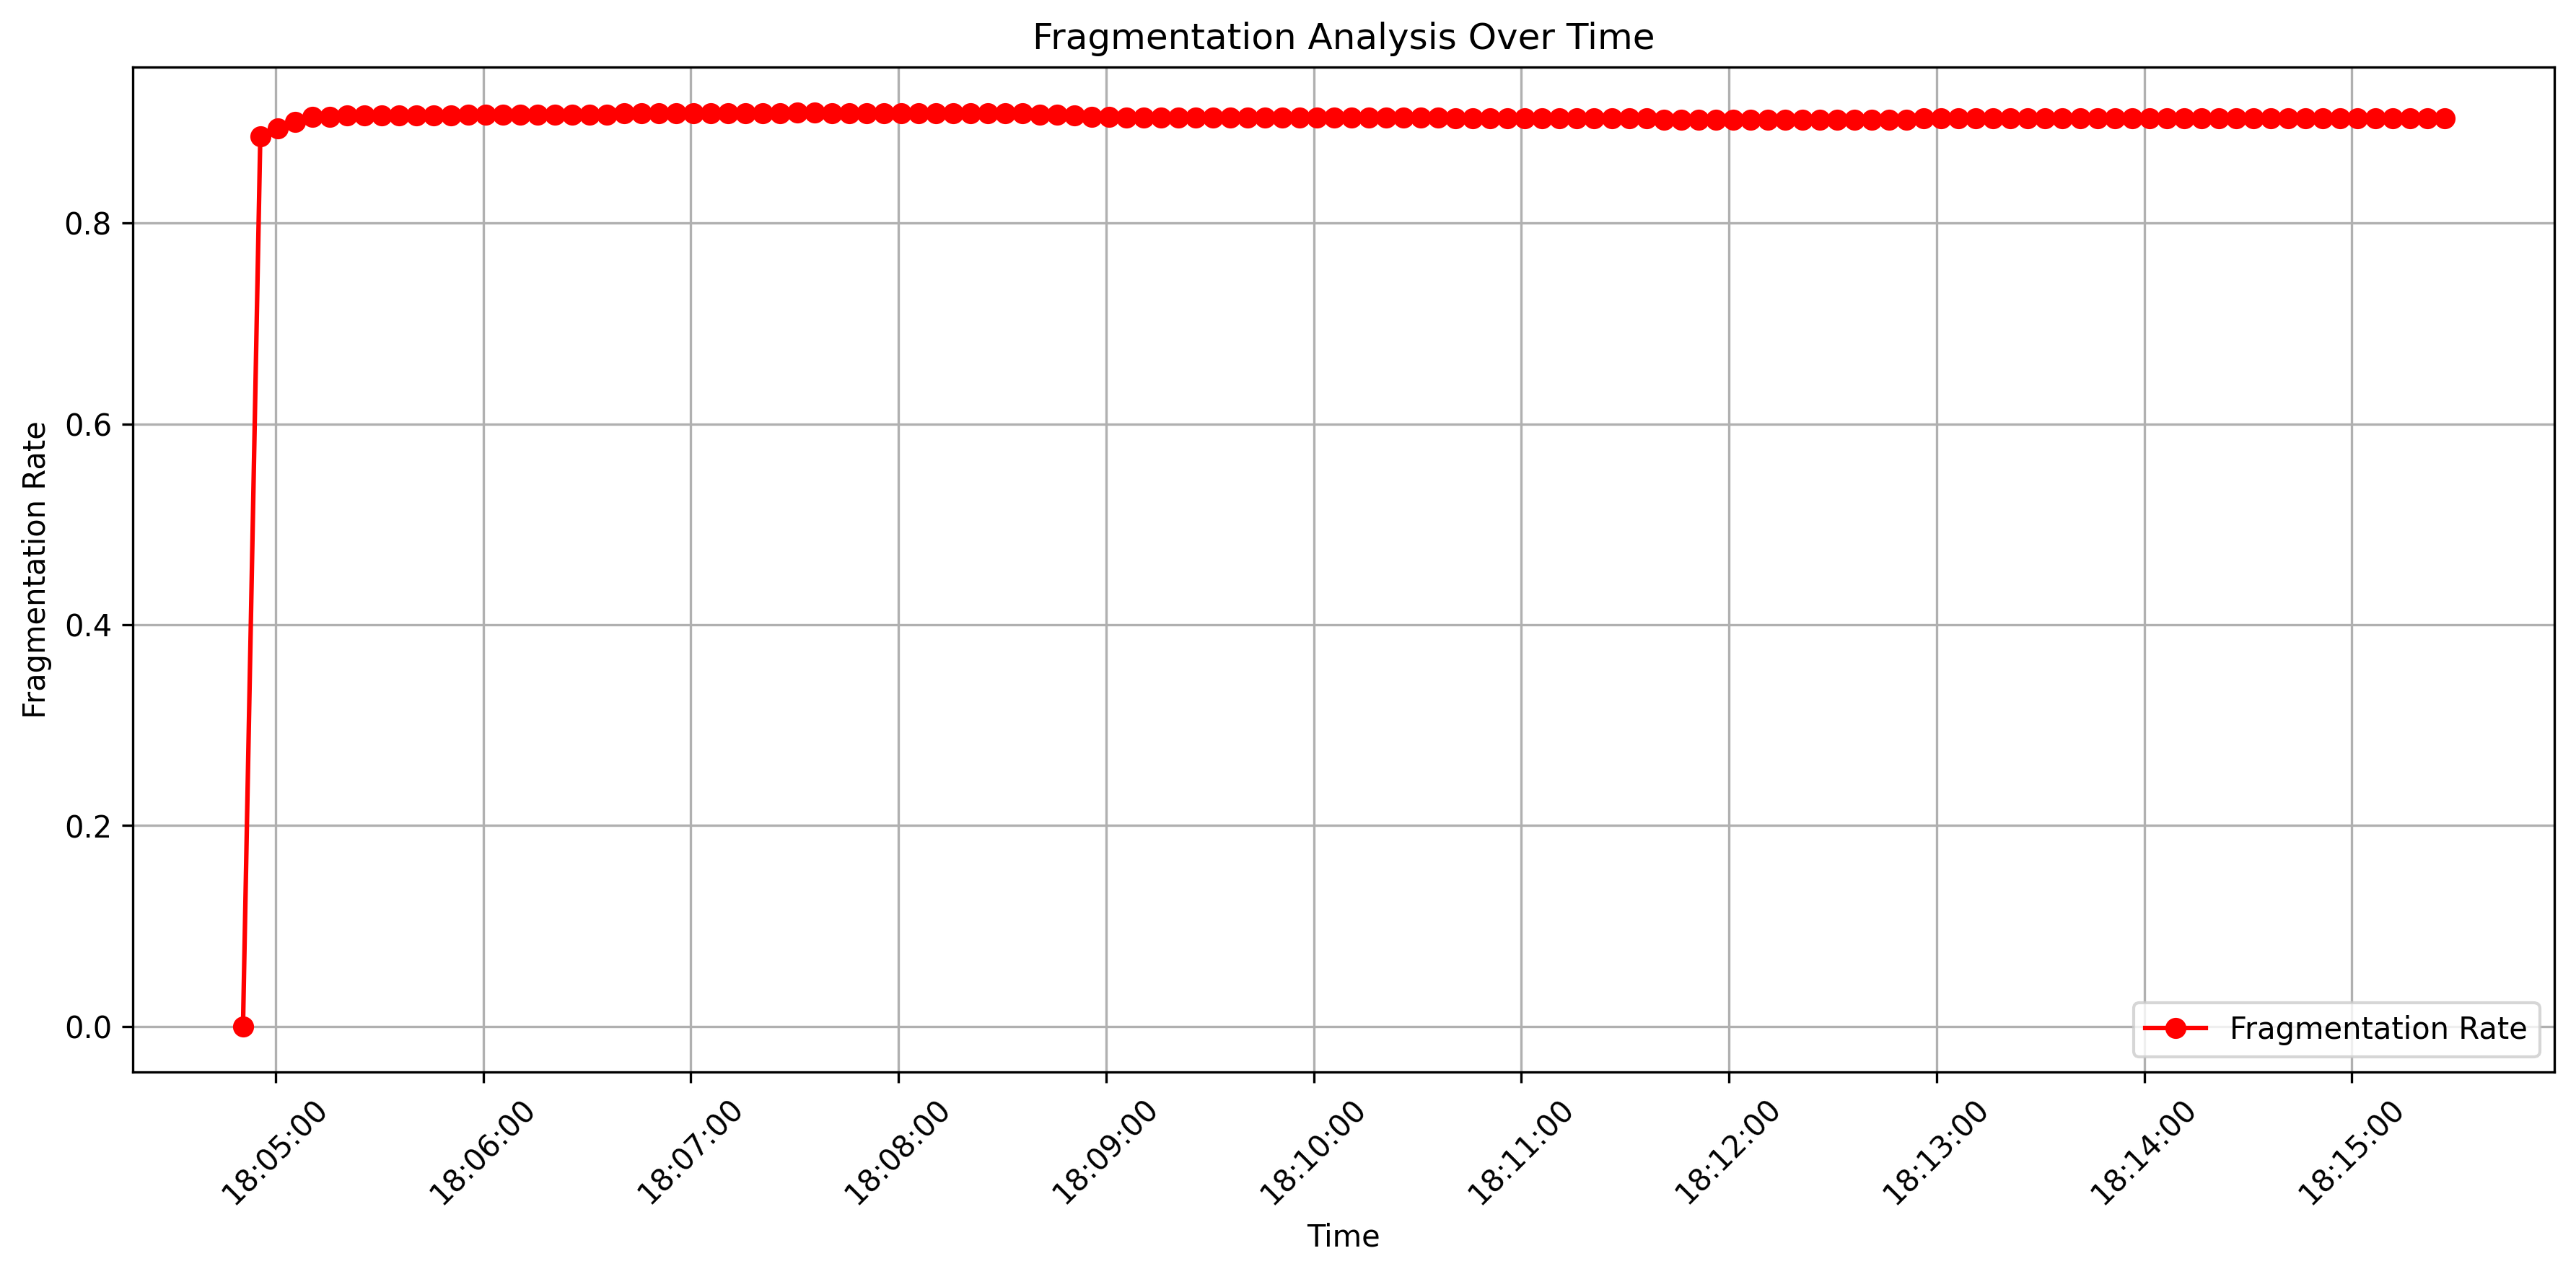
\includegraphics[width=0.8\textwidth]{Evaluation/single_fragmentation_analysis.png}
\caption{Single Client Fragmentation Rate vs Time}
\label{fig:fragmentation-analysis}
\end{figure}

Figure~\ref{fig:fragmentation-analysis} shows the fragmentation behavior throughout the session from 18:05 to 18:15. The fragmentation rate stabilizes at approximately 0.9 (90\%), significantly exceeding the configured threshold of 0.5 (50\%), triggering high fragmentation warnings. Despite this, the system maintained stable performance without degradation in throughput or latency.
The high fragmentation rate is primarily due to the large size of the input data. Media packets, including video streams with substantial frame data and audio packets with buffers of 4096 samples, often exceed the 3000-byte datagram size limit, necessitating fragmentation. These oversized payloads are split across multiple packets, which is expected given the nature of the data streams.



\subsubsection{Throughput Performance}

\begin{figure}[h!]
\centering
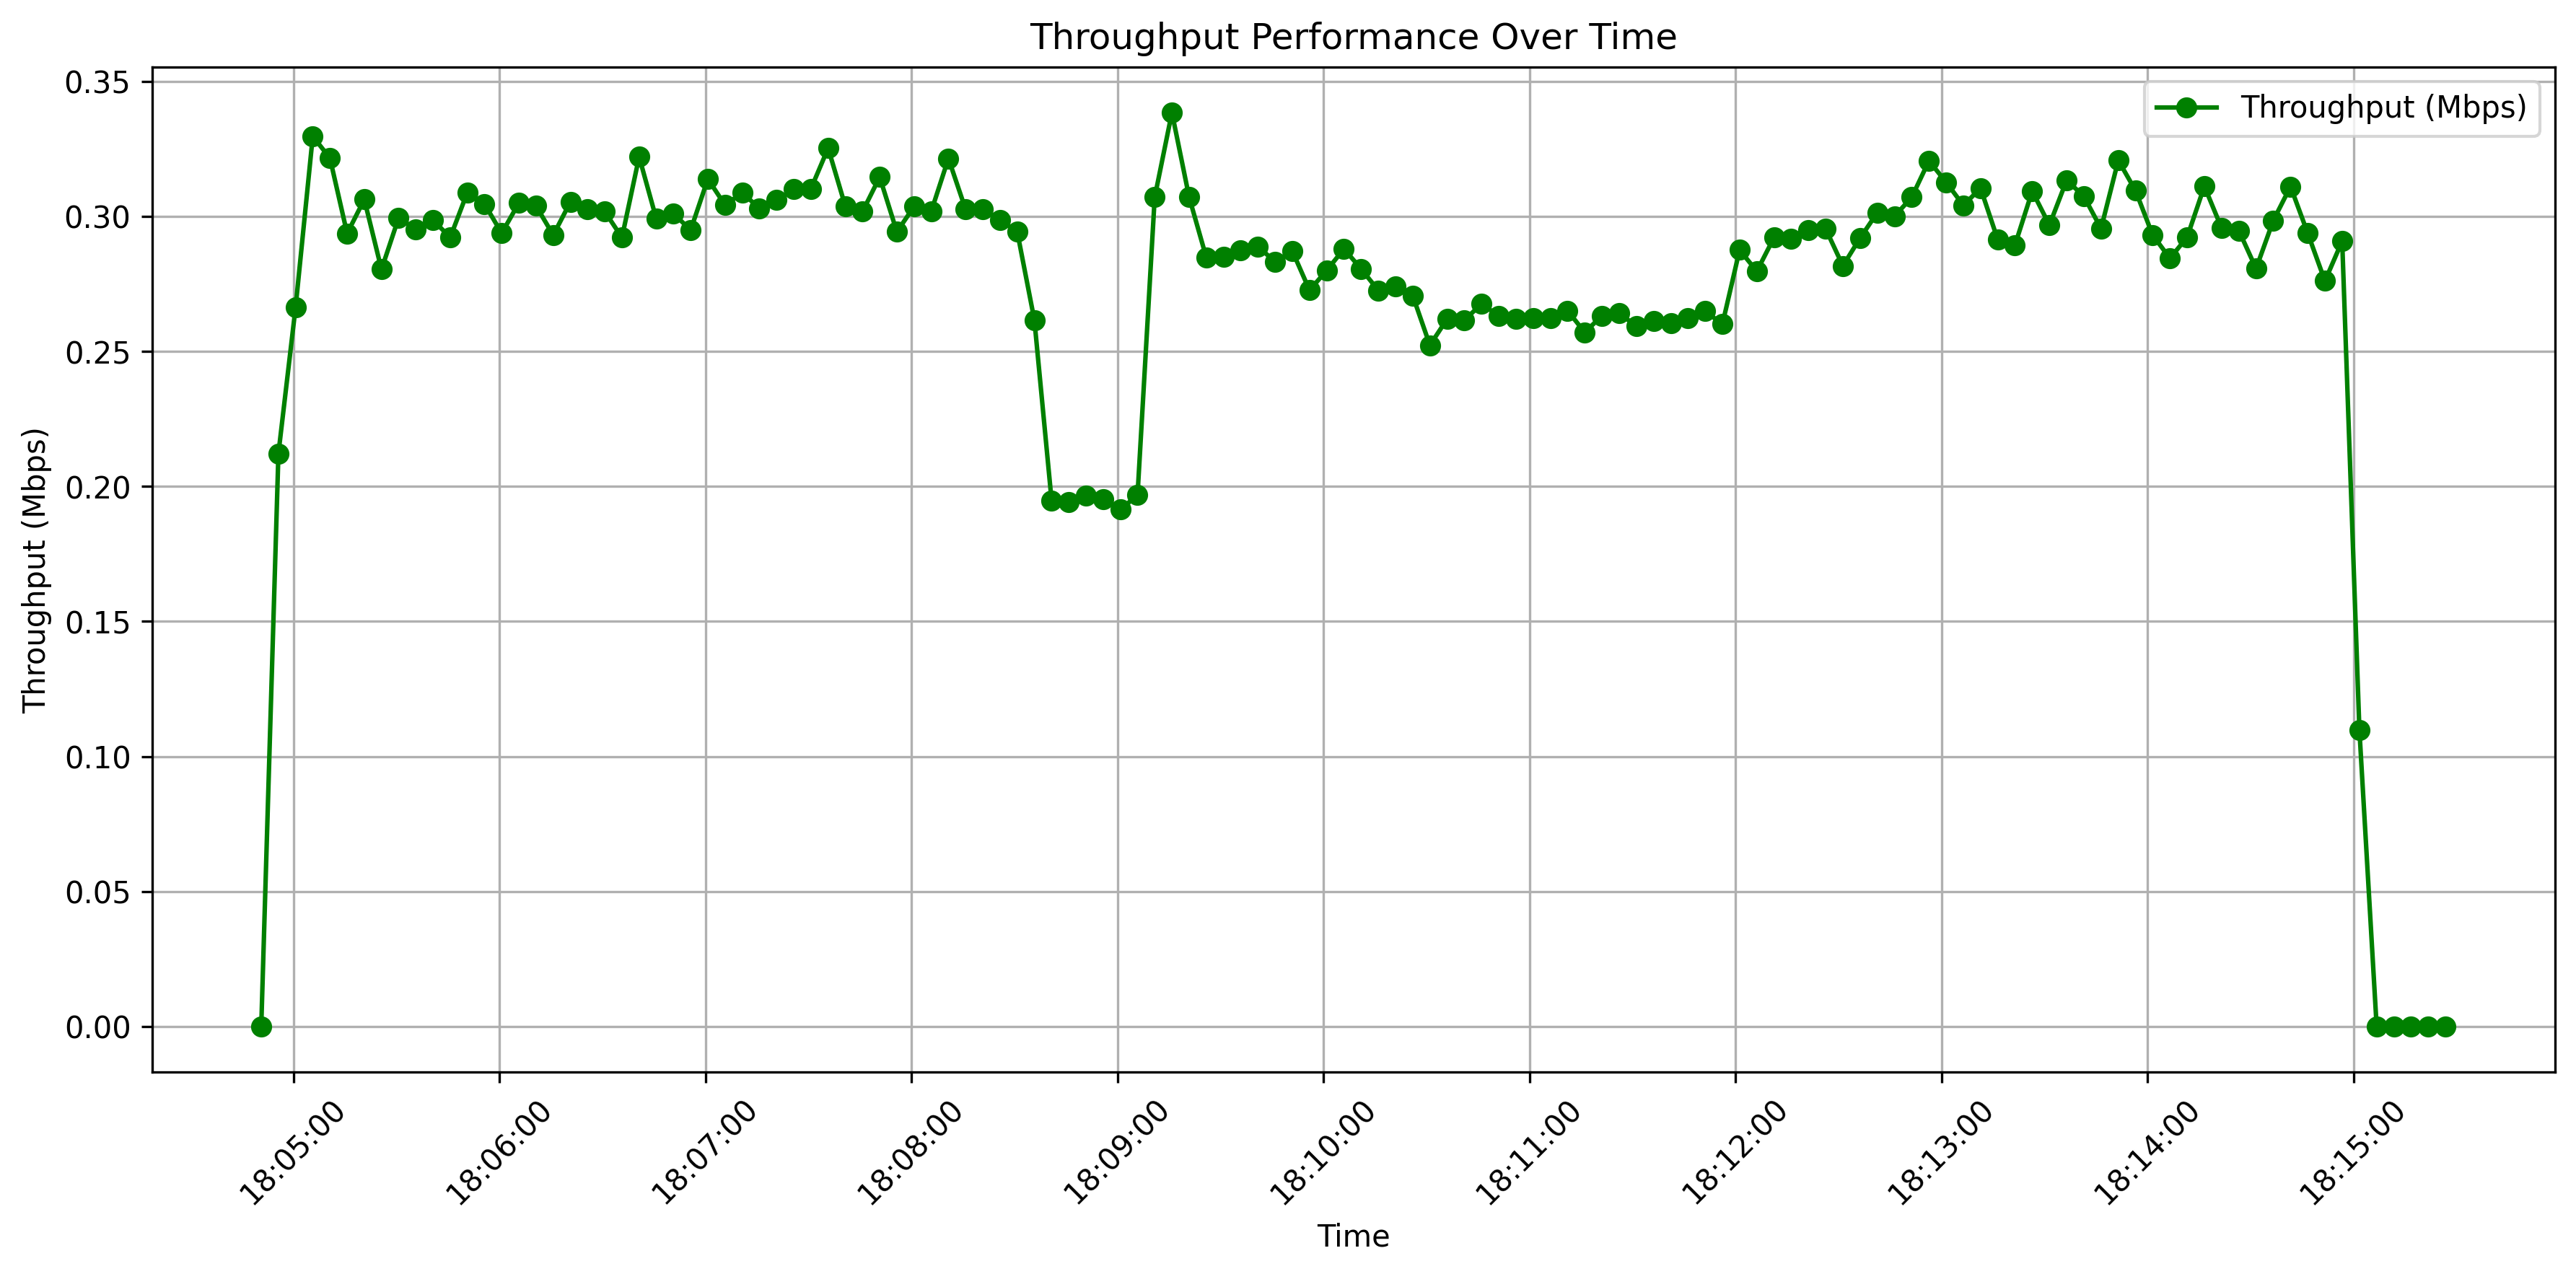
\includegraphics[width=0.8\textwidth]{Evaluation/single_throughput_performance.png}
\caption{Single Client Throughput vs Time}
\label{fig:single-throughput-performance}
\end{figure}

Figure~\ref{fig:single-throughput-performance} displays the throughput performance over time from 18:05 to 18:15. The system maintained a throughput ranging between 0.25 and 0.35 Mbps, with a peak performance of approximately 0.35 Mbps around 18:06-18:07. The throughput declined sharply to 0.0 Mbps at 18:15, corresponding to the session termination.
The throughput analysis indicates an average throughput of about 0.28 Mbps, with variations showing a ±25\% fluctuation from the average. The initial rise to 0.35 Mbps suggests high data handling capacity early in the session, while the dip around 18:08-18:09 reflects a temporary reduction, possibly due to processing adjustments. The decline to 0.0 Mbps at 18:15 shows graceful connection termination without any form of interruptions.


\subsubsection{Latency and Processing Time}
The system showcased excellent latency performance, with an average processing time of just 0.03-0.04 milliseconds which remained consistent throughout the session. Similarly, the average buffer wait time was also 0.03-0.04 milliseconds, indicating minimal queuing and efficient data handling. Notably, latency remained stable and showed no observable correlation with fluctuations in throughput or packet fragmentation.

These low latency values confirm the system's suitability for real-time applications requiring minimal processing delays.

\subsubsection{Buffer Management}
Buffer management for \texttt{client\_134025892847376}, as recorded in the \texttt{buffer\_metrics\allowbreak{}\_20250805\_180450.csv} log between 18:05 and 18:15 on August 5, 2025, demonstrates effective handling of dynamic data loads. The buffer size \texttt{buffer\_size\_bytes} varied throughout the session, occasionally dropping to 0 bytes and peaking at 13{,}398 bytes. Initially, the maximum buffer capacity \texttt{max\_buffer\_size\_bytes} remained constant at 21{,}475 bytes until 18:08:35, after which it increased to 24{,}281 bytes, indicating an adaptive strategy to accommodate increased data traffic. Notably, no buffer overflows \texttt{buffer\_overflows} were recorded, reflecting the system’s robust buffer allocation and the ability to absorb traffic fluctuations without packet loss.

\subsection{Three-Client Performance Analysis}
The three-client experiment characterizes the WebTransport router under a moderate, multi-tenant load.
\begin{figure}[h!]
\centering
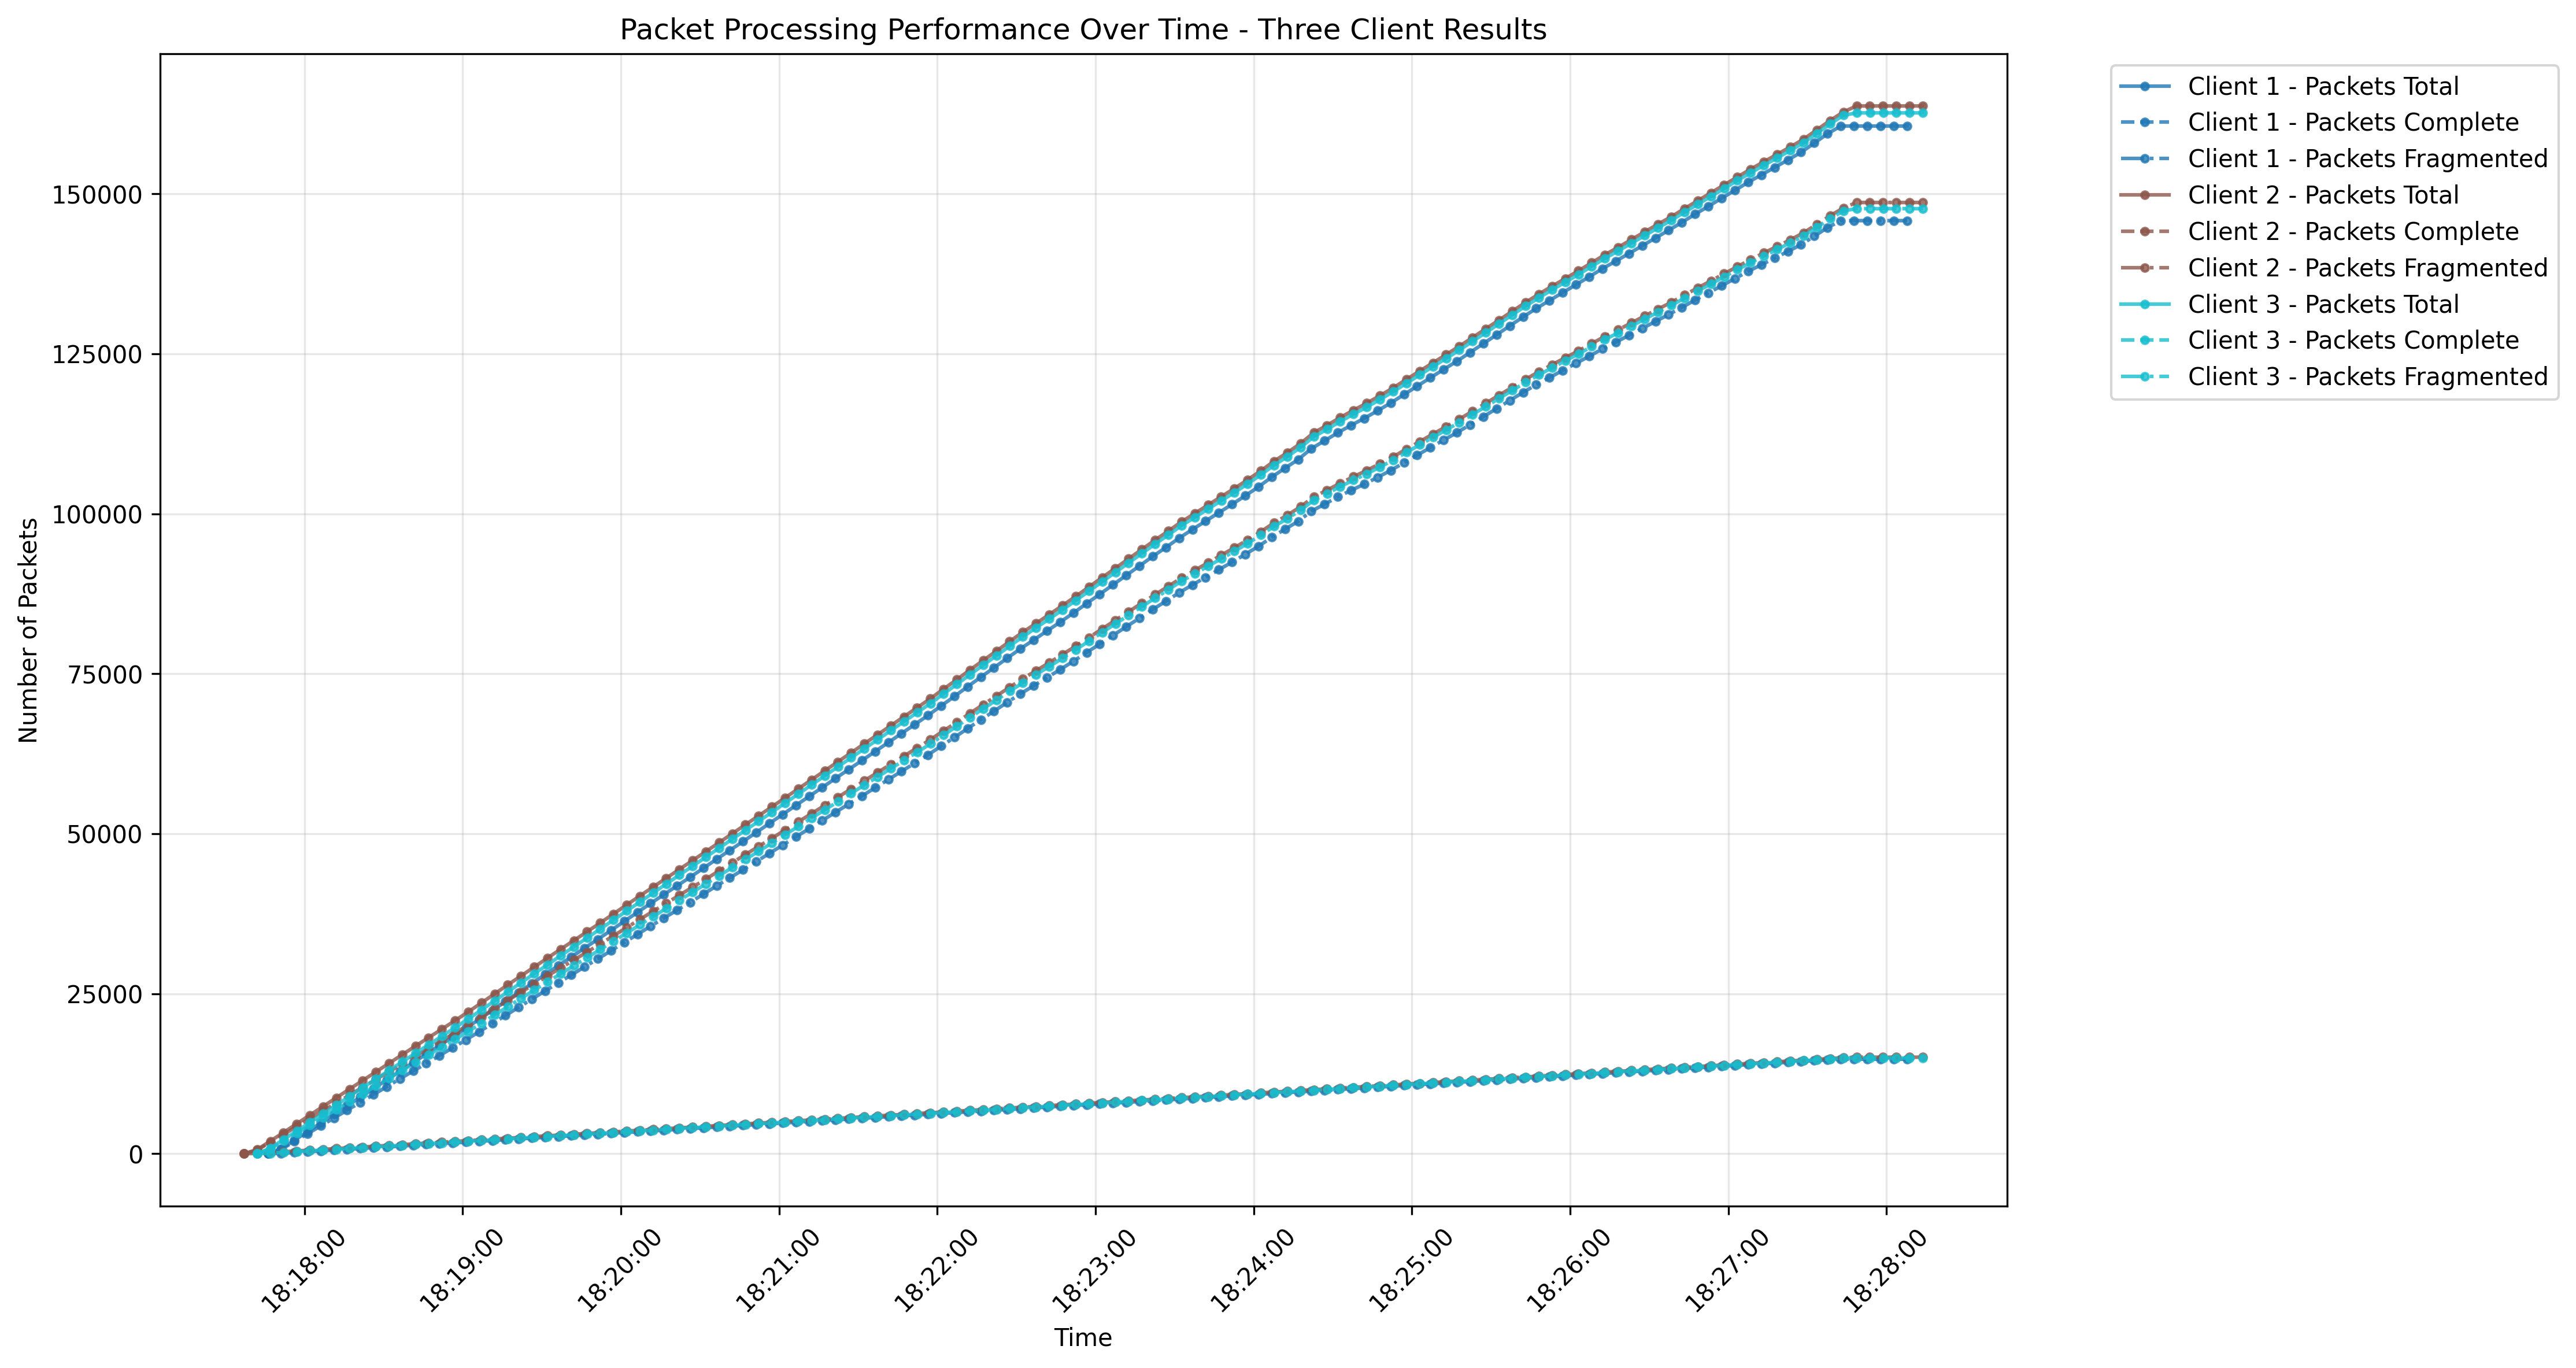
\includegraphics[width=0.8\textwidth]{Evaluation/packet_processing_by_client_three-client-results.png}
\caption{Packet Processing Performance Over Time – Three Client Results}
\label{fig:packet-processing-three-clients}
\end{figure}
Figure~\ref{fig:packet-processing-three-clients} illustrates the packet processing performance across three clients from 18:05 to 18:15, with the router handling approximately 487,000 packets in total. Each client processed: Client 1 with 160,586 packets, Client 2 with 162,643 packets, and Client 3 with 163,724 packets. The per-second arrival rate was linear and nearly identical across clients, indicating fair scheduling. Fragmentation averaged 90.8\%, resulting in about 442,000 fragmented packets and 45,000 complete packets, with a 100\% successful reassembly rate and no logged losses.\

\subsubsection{Three Client Fragmentation Analysis}
\begin{figure}[h!]
\centering
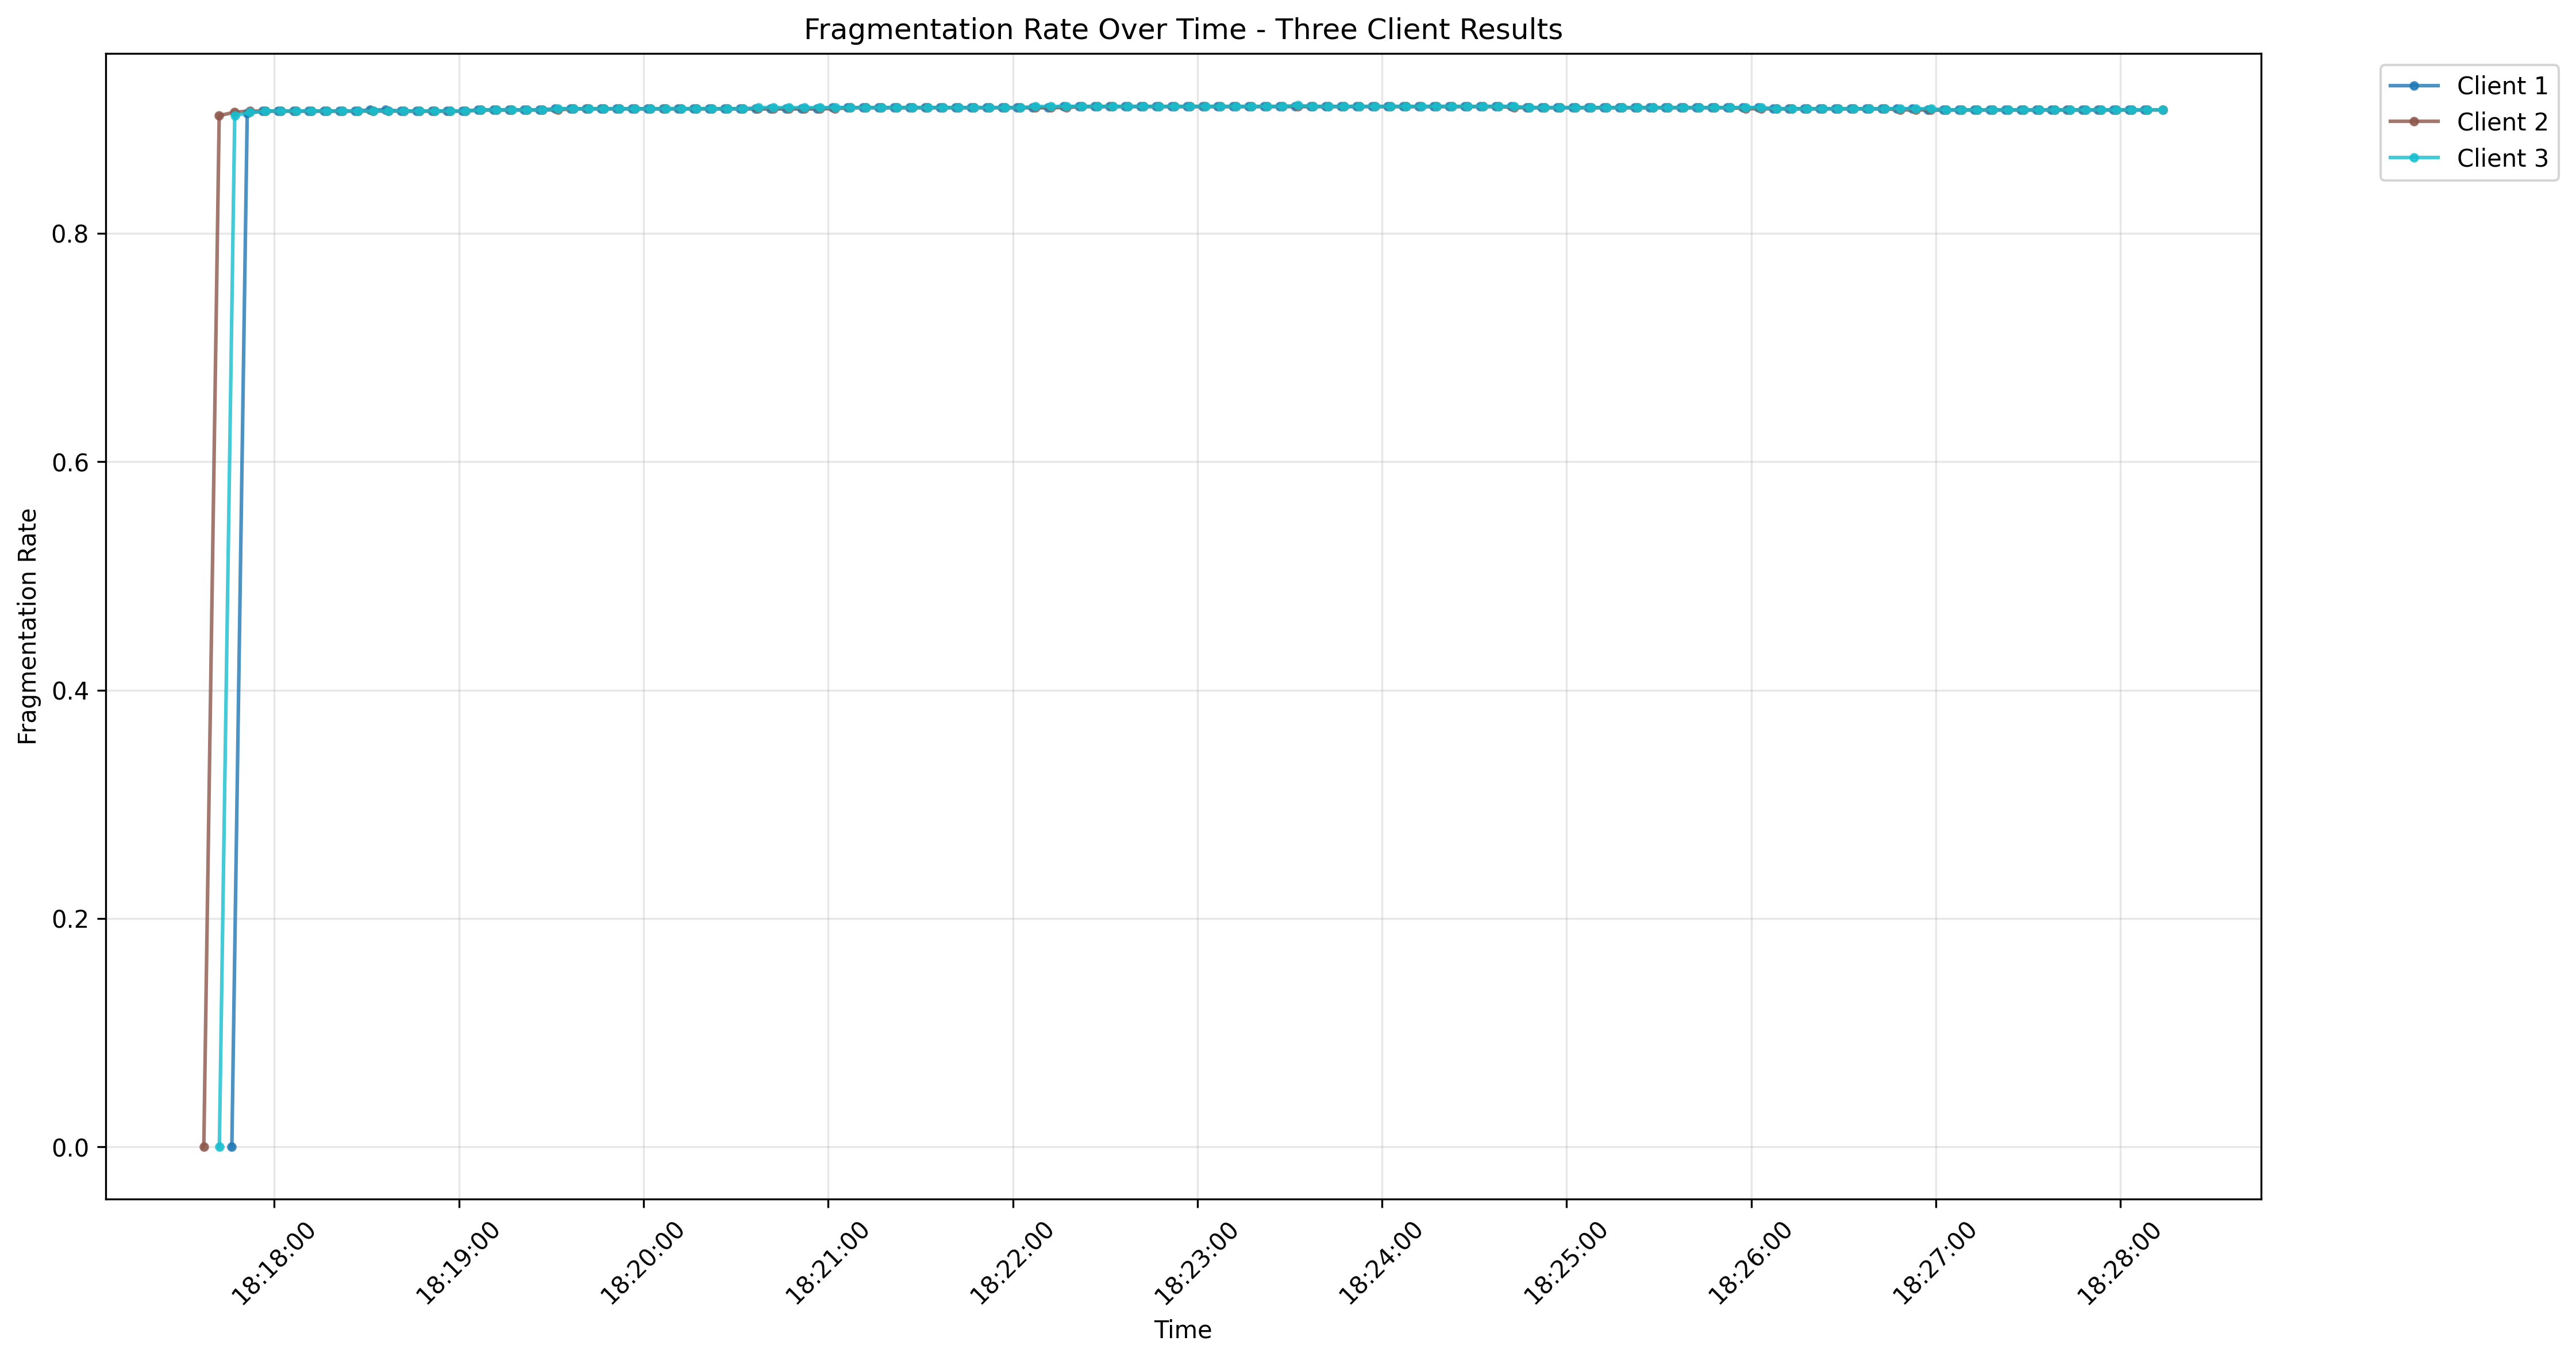
\includegraphics[width=0.8\textwidth]{Evaluation/fragmentation_by_client_three-client-results.png}
\caption{Fragmentation Rate Over Time – Three Client Results}
\label{fig:fragmentation-three-clients}
\end{figure}
Figure~\ref{fig:fragmentation-three-clients} shows the fragmentation behavior across the three clients, stabilizing at 0.9–0.91 (90–91\%), consistently exceeding the 0.5 (50\%) threshold and triggering high fragmentation warnings. The high rate is attributed to 4,096-sample audio buffers and large video frames surpassing the 3,000-byte datagram limit. Despite uniform 90\% fragmentation, throughput and latency remained stable, suggesting linear scalability in the fragmentation/reassembly path.


\subsubsection{Three Client Throughput Analysis}
\begin{figure}[h!]
\centering
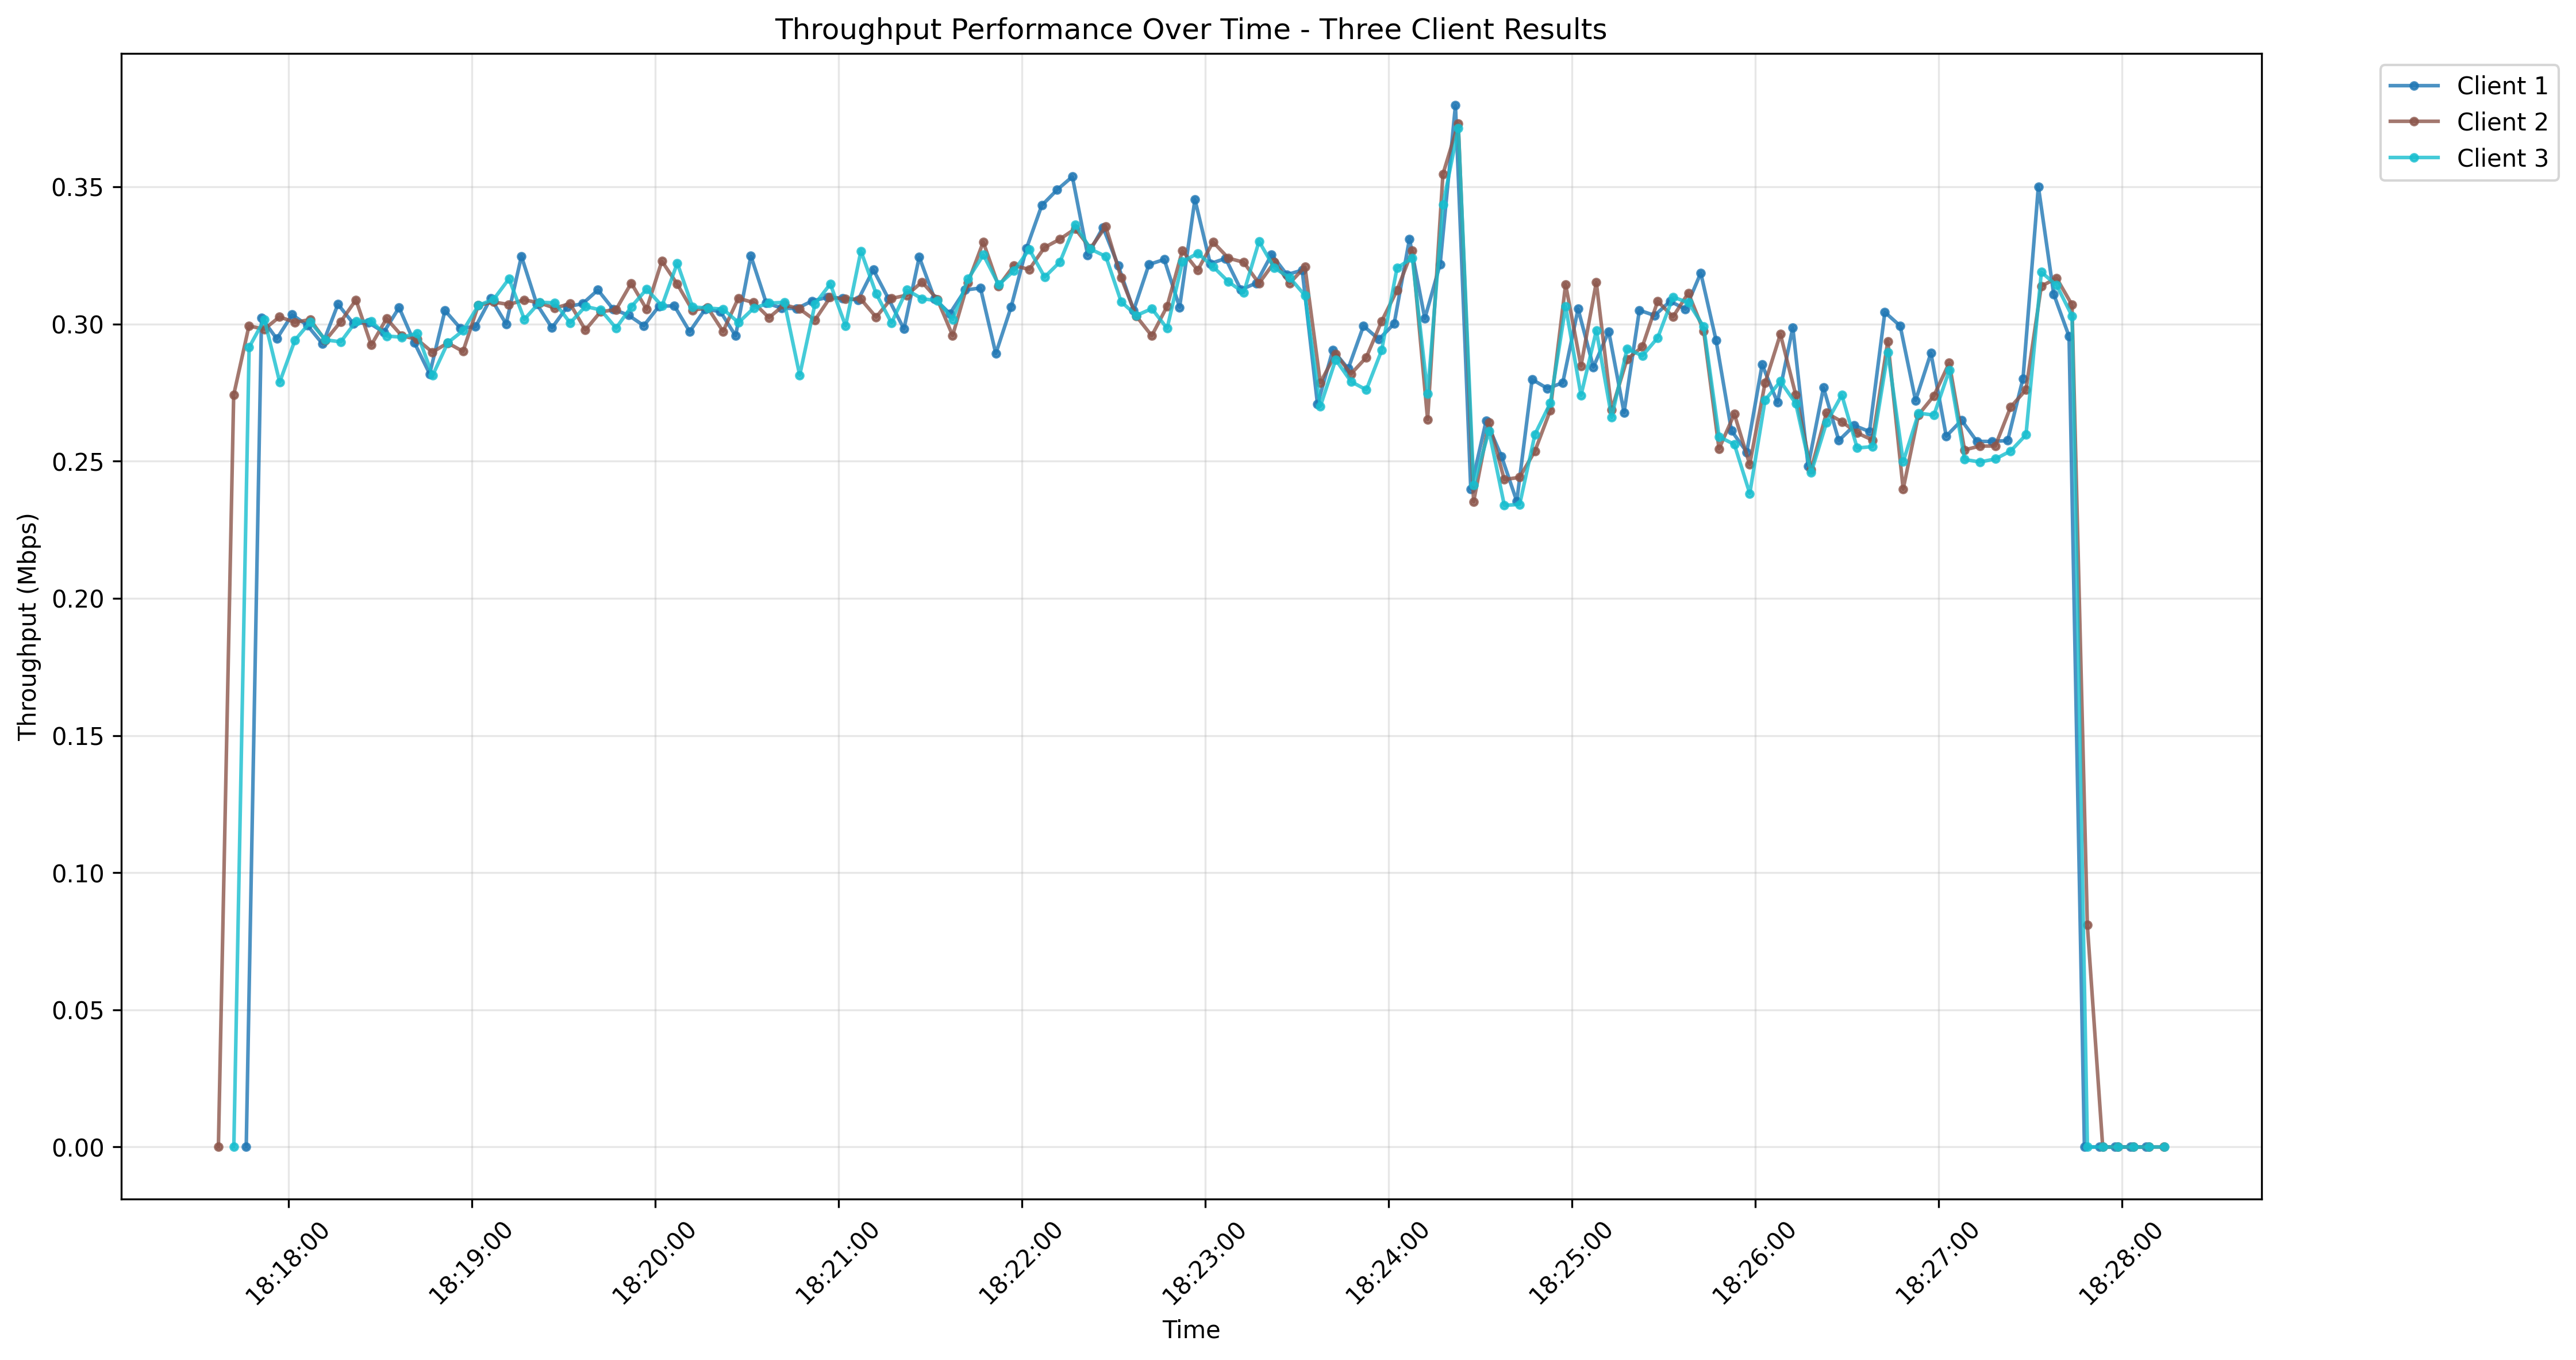
\includegraphics[width=0.8\textwidth]{Evaluation/throughput_by_client_three-client-results.png}
\caption{Throughput Over Time – Three Client Results}
\label{fig:throughput-three-clients}
\end{figure}
Figure~\ref{fig:throughput-three-clients} displays the throughput performance per client, with an average of 0.30 Mbps, an aggregate average of 0.90 Mbps, a peak of 0.38 Mbps, and a minimum of 0.23 Mbps. Throughput curves were smooth and uncorrelated, ruling out head-of-line blocking, with a brief dip to 0 Mbps at the end marking graceful connection teardown.

\begin{figure}[h!]
\centering
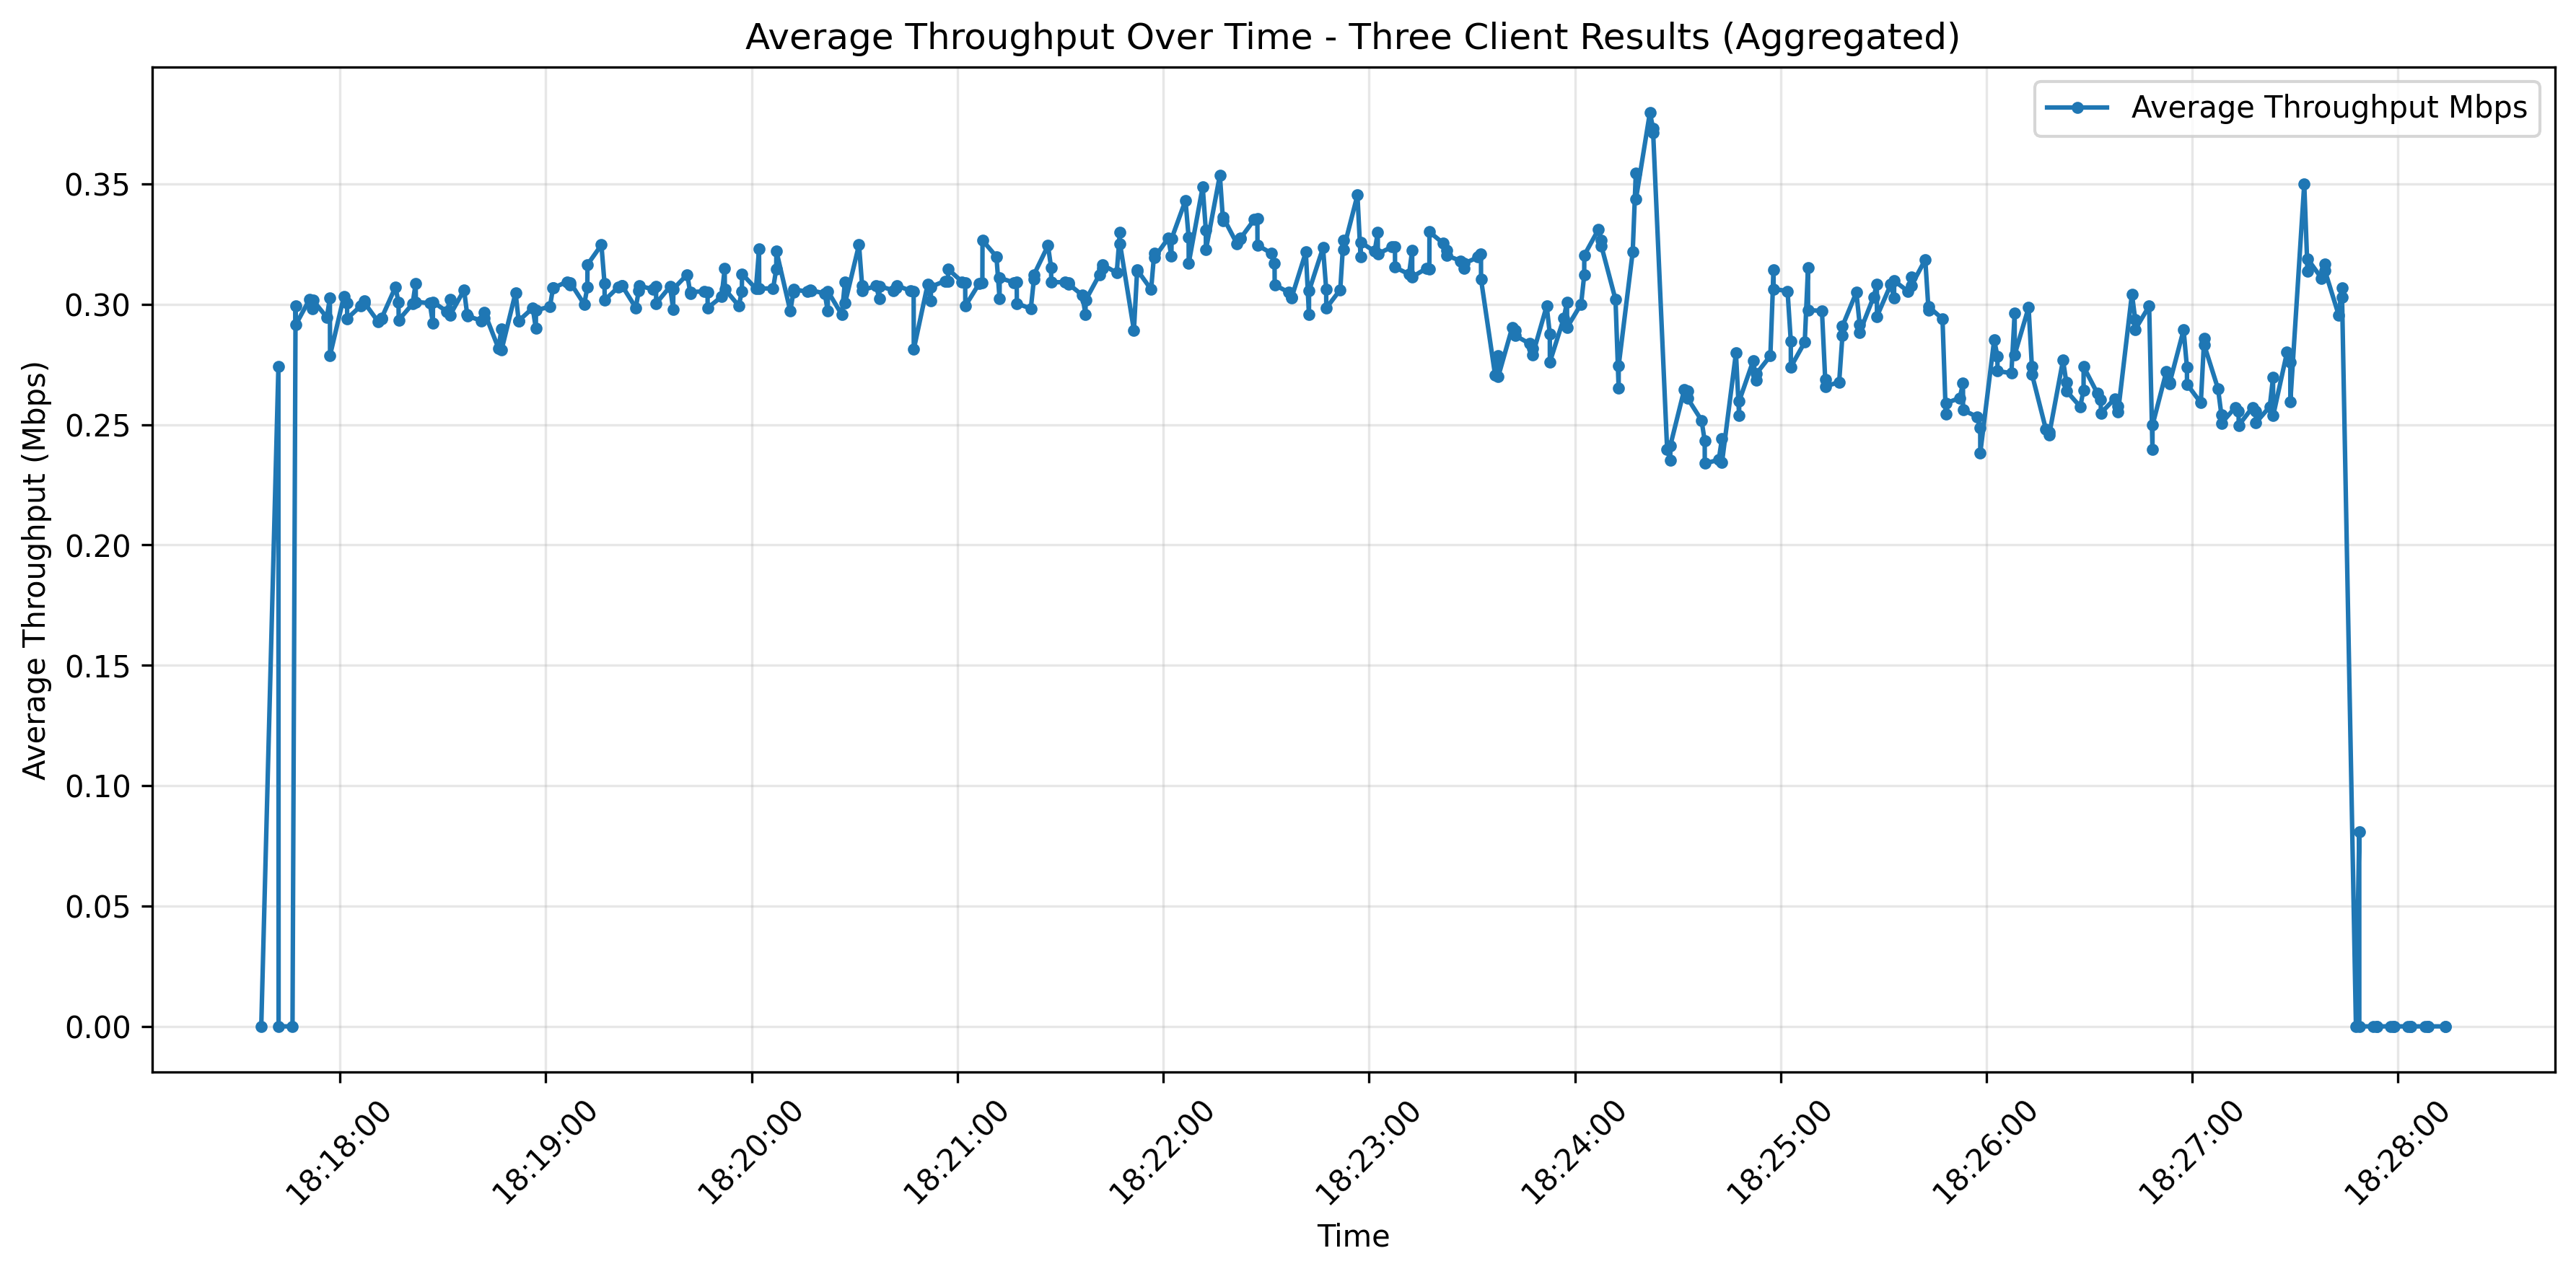
\includegraphics[width=0.8\textwidth]{Evaluation/avg_throughput_aggregated_three-client-results.png}
\caption{Average Aggregated Throughput}
\label{fig:avg-throughput-aggregated}
\end{figure}
Figure~\ref{fig:avg-throughput-aggregated} shows the combined throughput maintaining a steady 0.85–0.90 Mbps plateau, with no multi-second zero-throughput periods until deliberate shutdown.

\subsubsection{Router Pod Overview}
The router pod utilized 418 m (approximately 0.42 core) of CPU and 92 MiB of memory, with no restarts and stable performance throughout the 11-minute window, indicating modest control-plane and data-plane overhead for handling three clients.
\begin{figure}[h!]
\centering
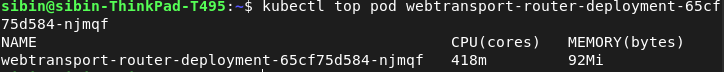
\includegraphics[width=0.8\textwidth]{Evaluation/three-clients-stats.png}
\caption{Router Pod Performance for 3 clients}
\label{fig:three-clients-stats}
\end{figure}

\subsubsection{Host Machine Overview}
The host machine showed CPU usage between 29.9\% and 40.6\% across cores (averaging around 35\%), memory usage at 8.53 GiB / 13.5 GiB (63\%), and a load of 2.85 / 2.16 / 2.04 with 308 tasks (2 running). Utilization was healthy with no swap thrashing, confirming adequate space.

\begin{figure}[h!]
\centering
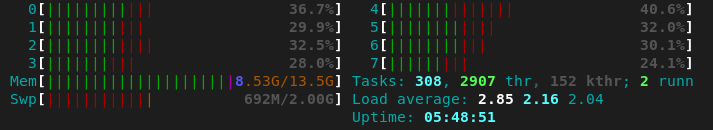
\includegraphics[width=0.8\textwidth]{Evaluation/three-clients-host-stats.png}
\caption{Host Machine stats for 3 clients}
\label{fig:three-clients-host-stats}
\end{figure}

\subsubsection{Latency and Processing Time}
Latency remained sub-millisecond, with an average processing time of 0.02–0.04 ms and an average buffer wait time of 0.02–0.04 ms across all clients, indicating no increase in per-packet overhead with additional concurrent clients.
\subsubsection{Buffer Management}
Each client maintained an independent buffer ring, with the maximum buffer size auto-tuning from 16–17 kB to 24 kB as traffic increased. Peak usage reached 18,270 bytes (Client 1), well below the 24 kB limit, and no buffer overflows were recorded, demonstrating effective back-pressure and kernel socket buffer management


\subsection{Five-Client Performance Analysis}
The five-client experiment extends the scaling study to 15 concurrent media streams (5 clients × 3 streams each) and represents the first high-load scenario for the WebTransport router \cite{rfc9000}.

\subsubsection{Five-Client Packet Processing Performance}

\begin{figure}[H]
\centering
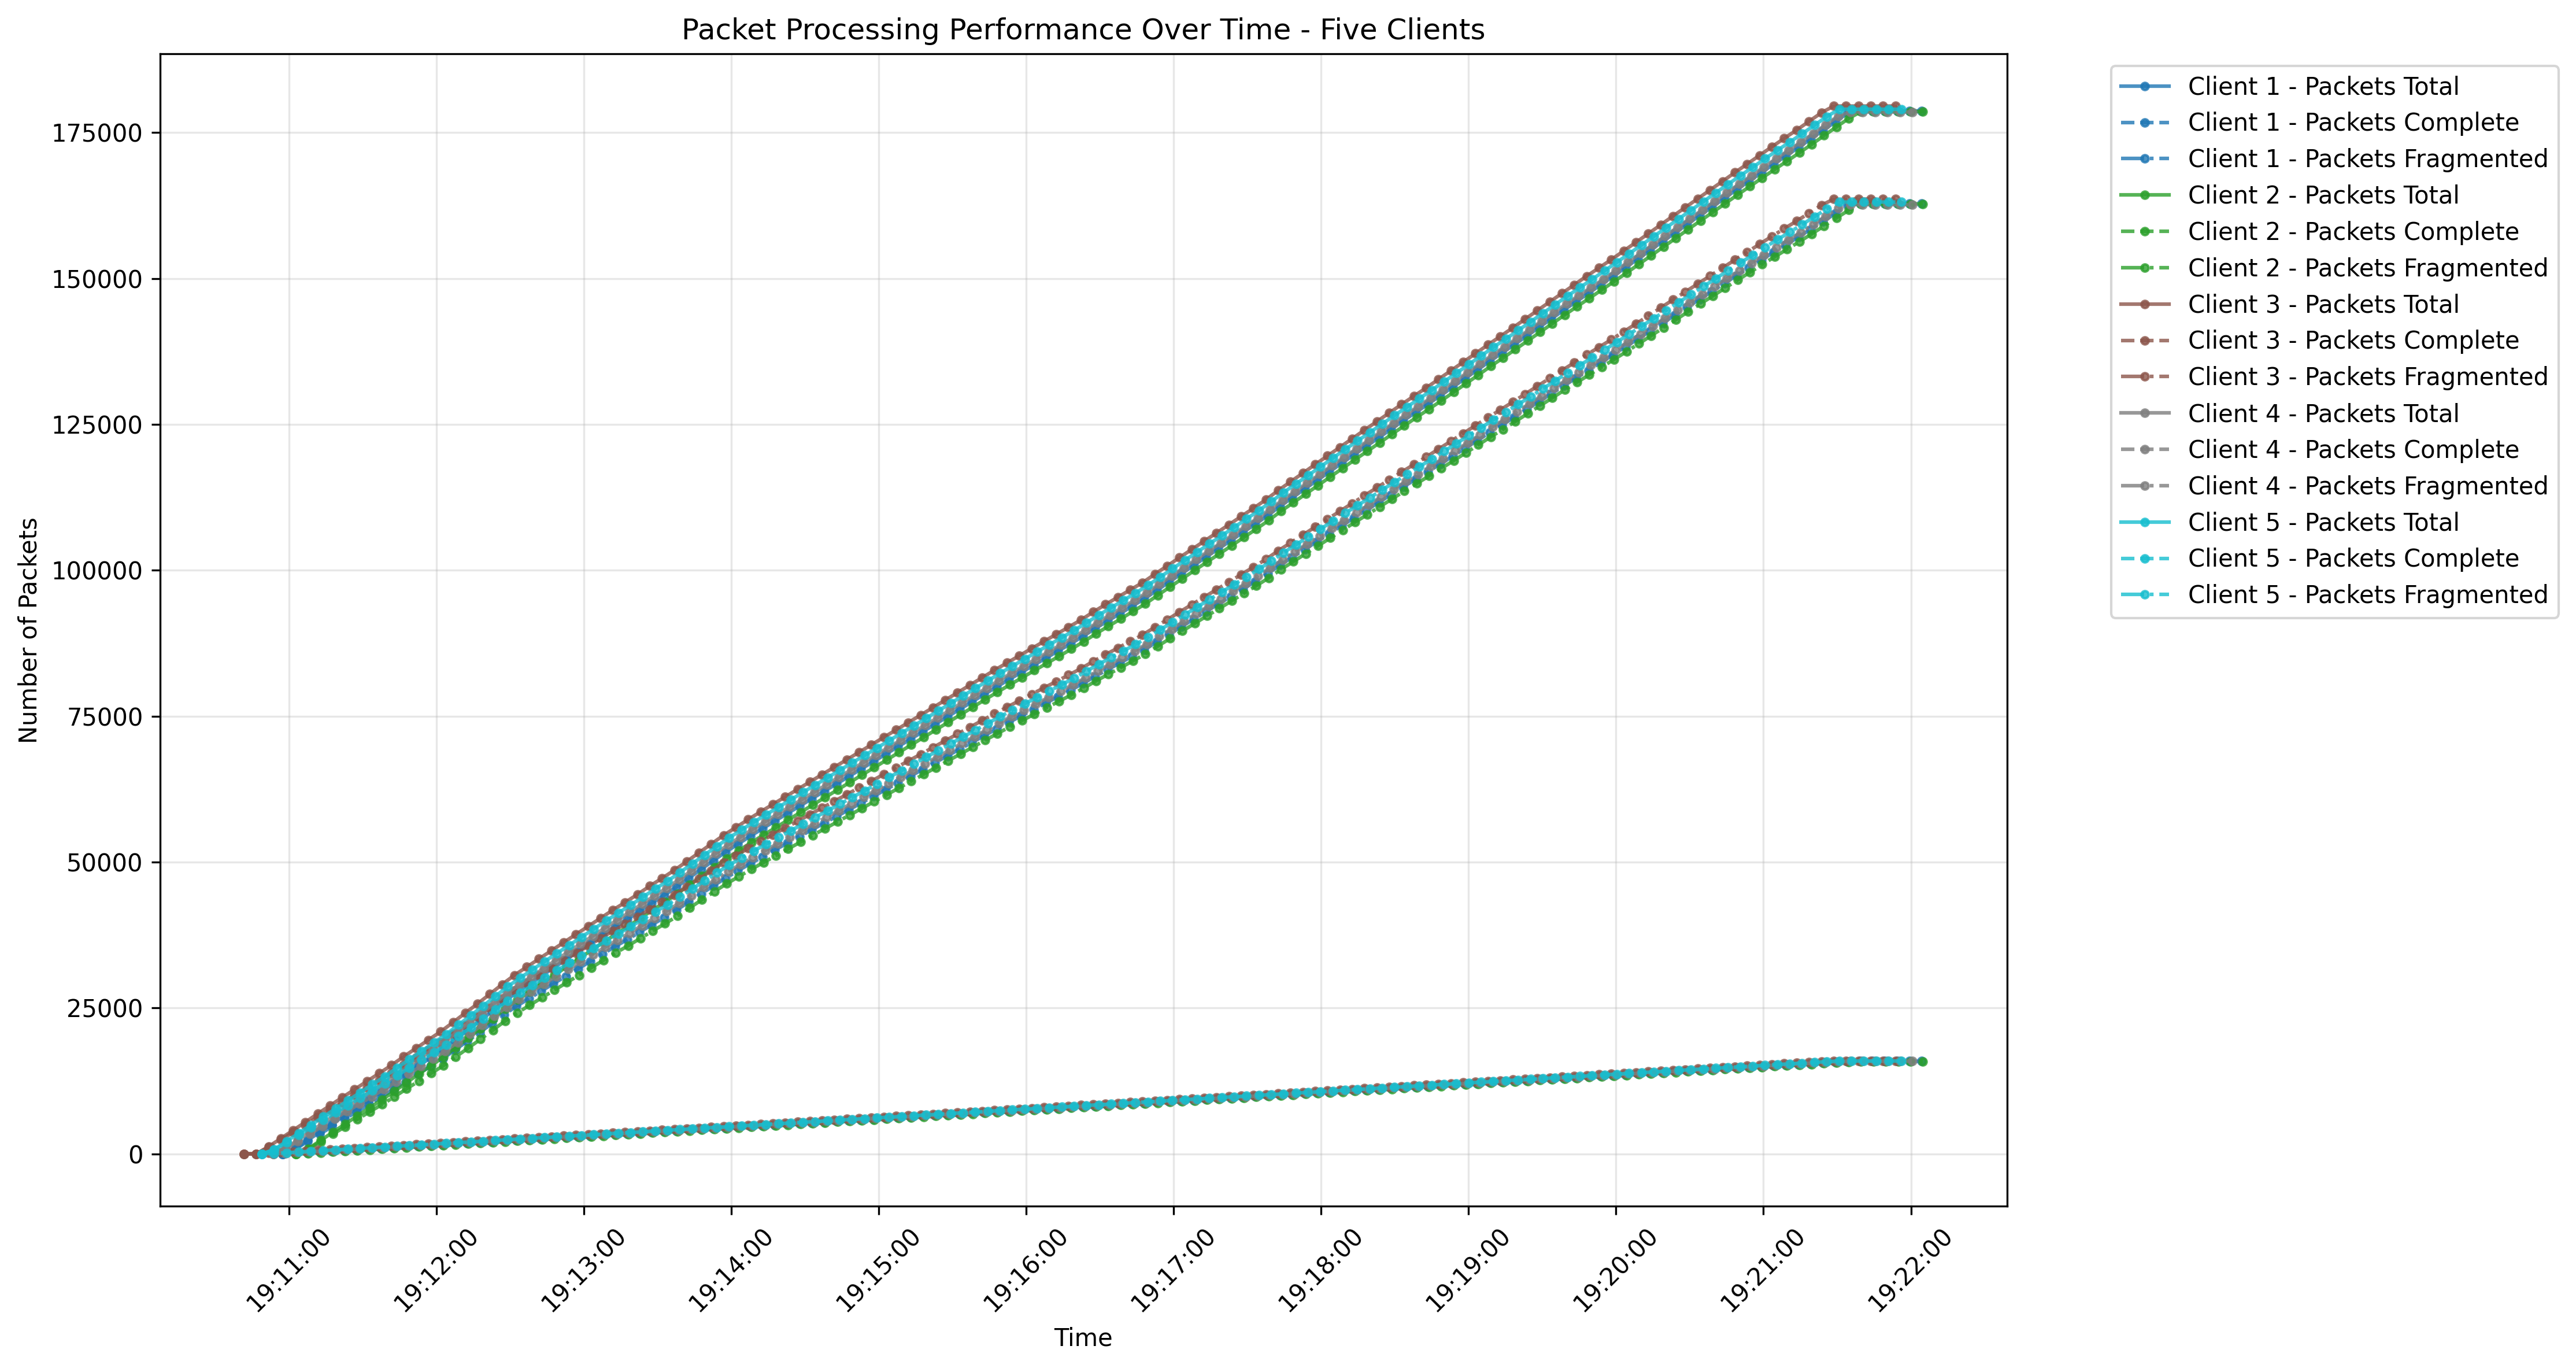
\includegraphics[width=0.8\textwidth]{Evaluation/packet_processing_by_client_five-clients.png}
\caption{Packet Processing – Five Clients}
\label{fig:packet-processing-five-clients}
\end{figure}

Figure~\ref{fig:packet-processing-five-clients} illustrates the packet processing performance across five clients from start 19:10 to end 19:22 on August 5, 2025, processing an aggregate of approximately 890,000 packets. The individual client packet counts ranged from 175,000 to 180,000, which showed linear growth and fair scheduling without head-of-line blocking \cite{rfc9000}. The fragmentation rate varied between 90.8\% and 91.6\%, with 100\% reassembly success and no packet losses.

\subsubsection{Five-Client Fragmentation Analysis}

\begin{figure}[H]
\centering
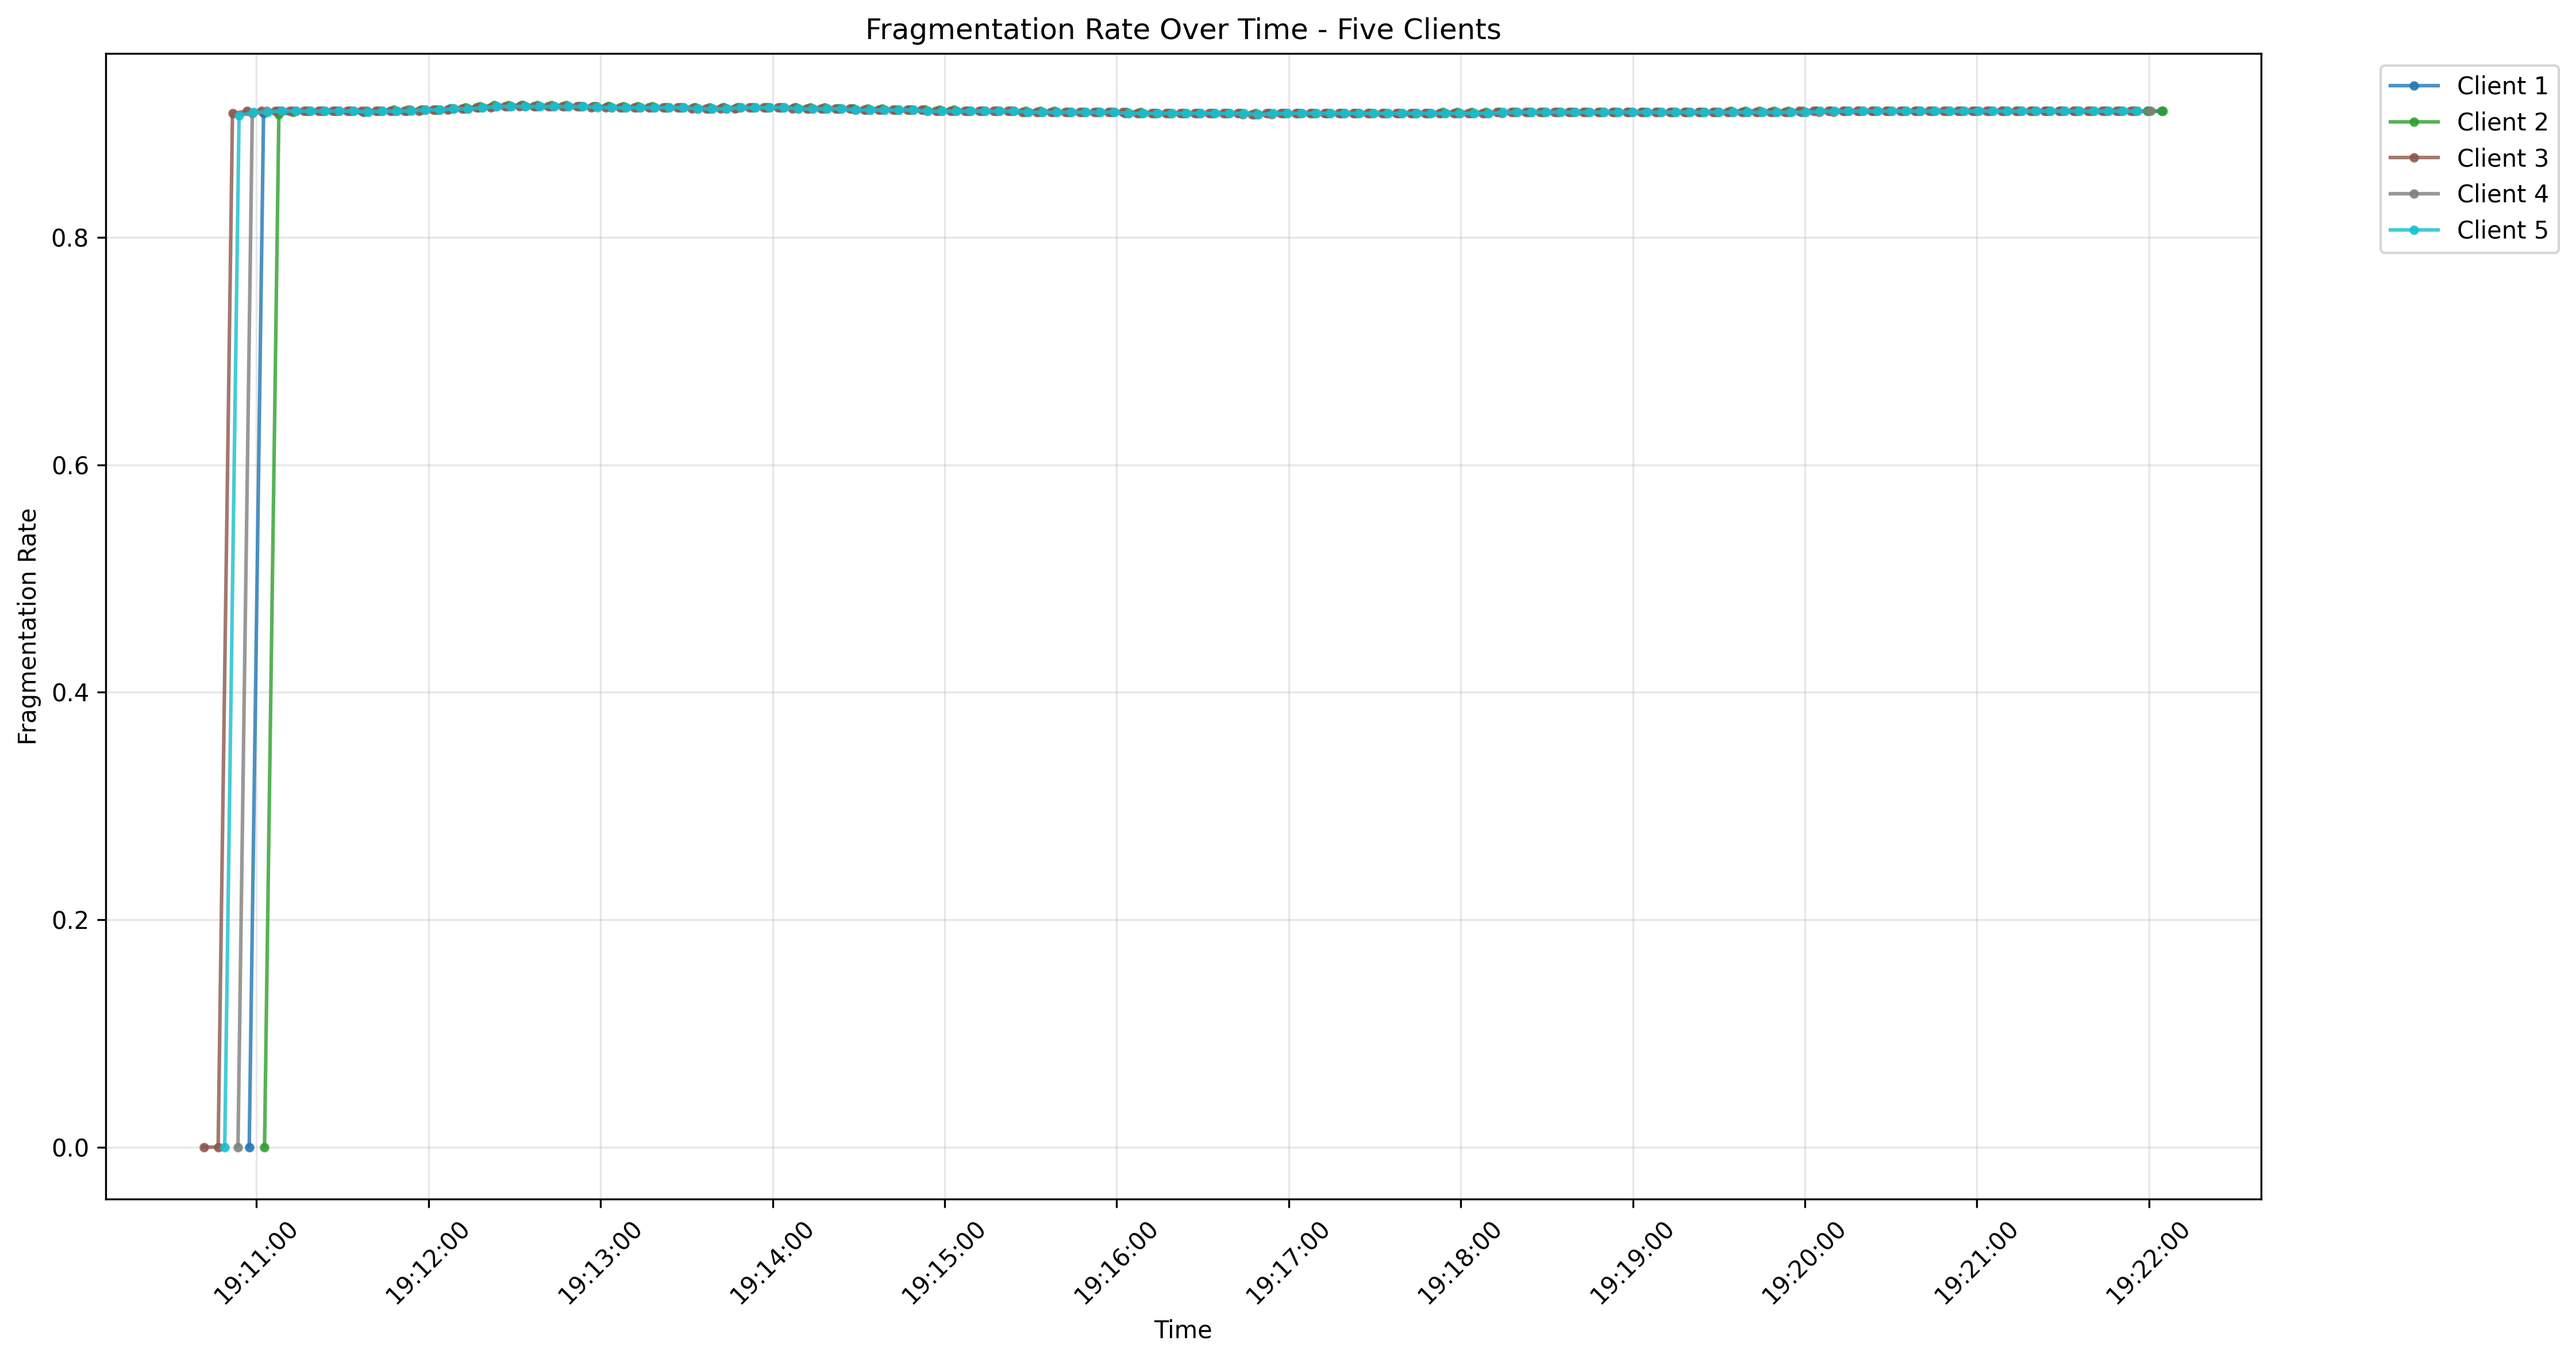
\includegraphics[width=0.8\textwidth]{Evaluation/fragmentation_by_client_five-clients.png}
\caption{Fragmentation Rate – Five Clients}
\label{fig:fragmentation-five-clients}
\end{figure}

Figure~\ref{fig:fragmentation-five-clients} displays the fragmentation behavior across the five clients, stabilizing at approximately 0.9 (90\%), consistently triggering HIGH\_FRAGMENTATION warnings. The high rate is due to 4,096-sample audio buffers and large video frames exceeding the 3,000-byte datagram limit, yet throughput and latency remained unaffected, highlighting efficient reassembly.

\subsubsection{Five-Client Throughput Analysis}

\begin{figure}[H]
\centering
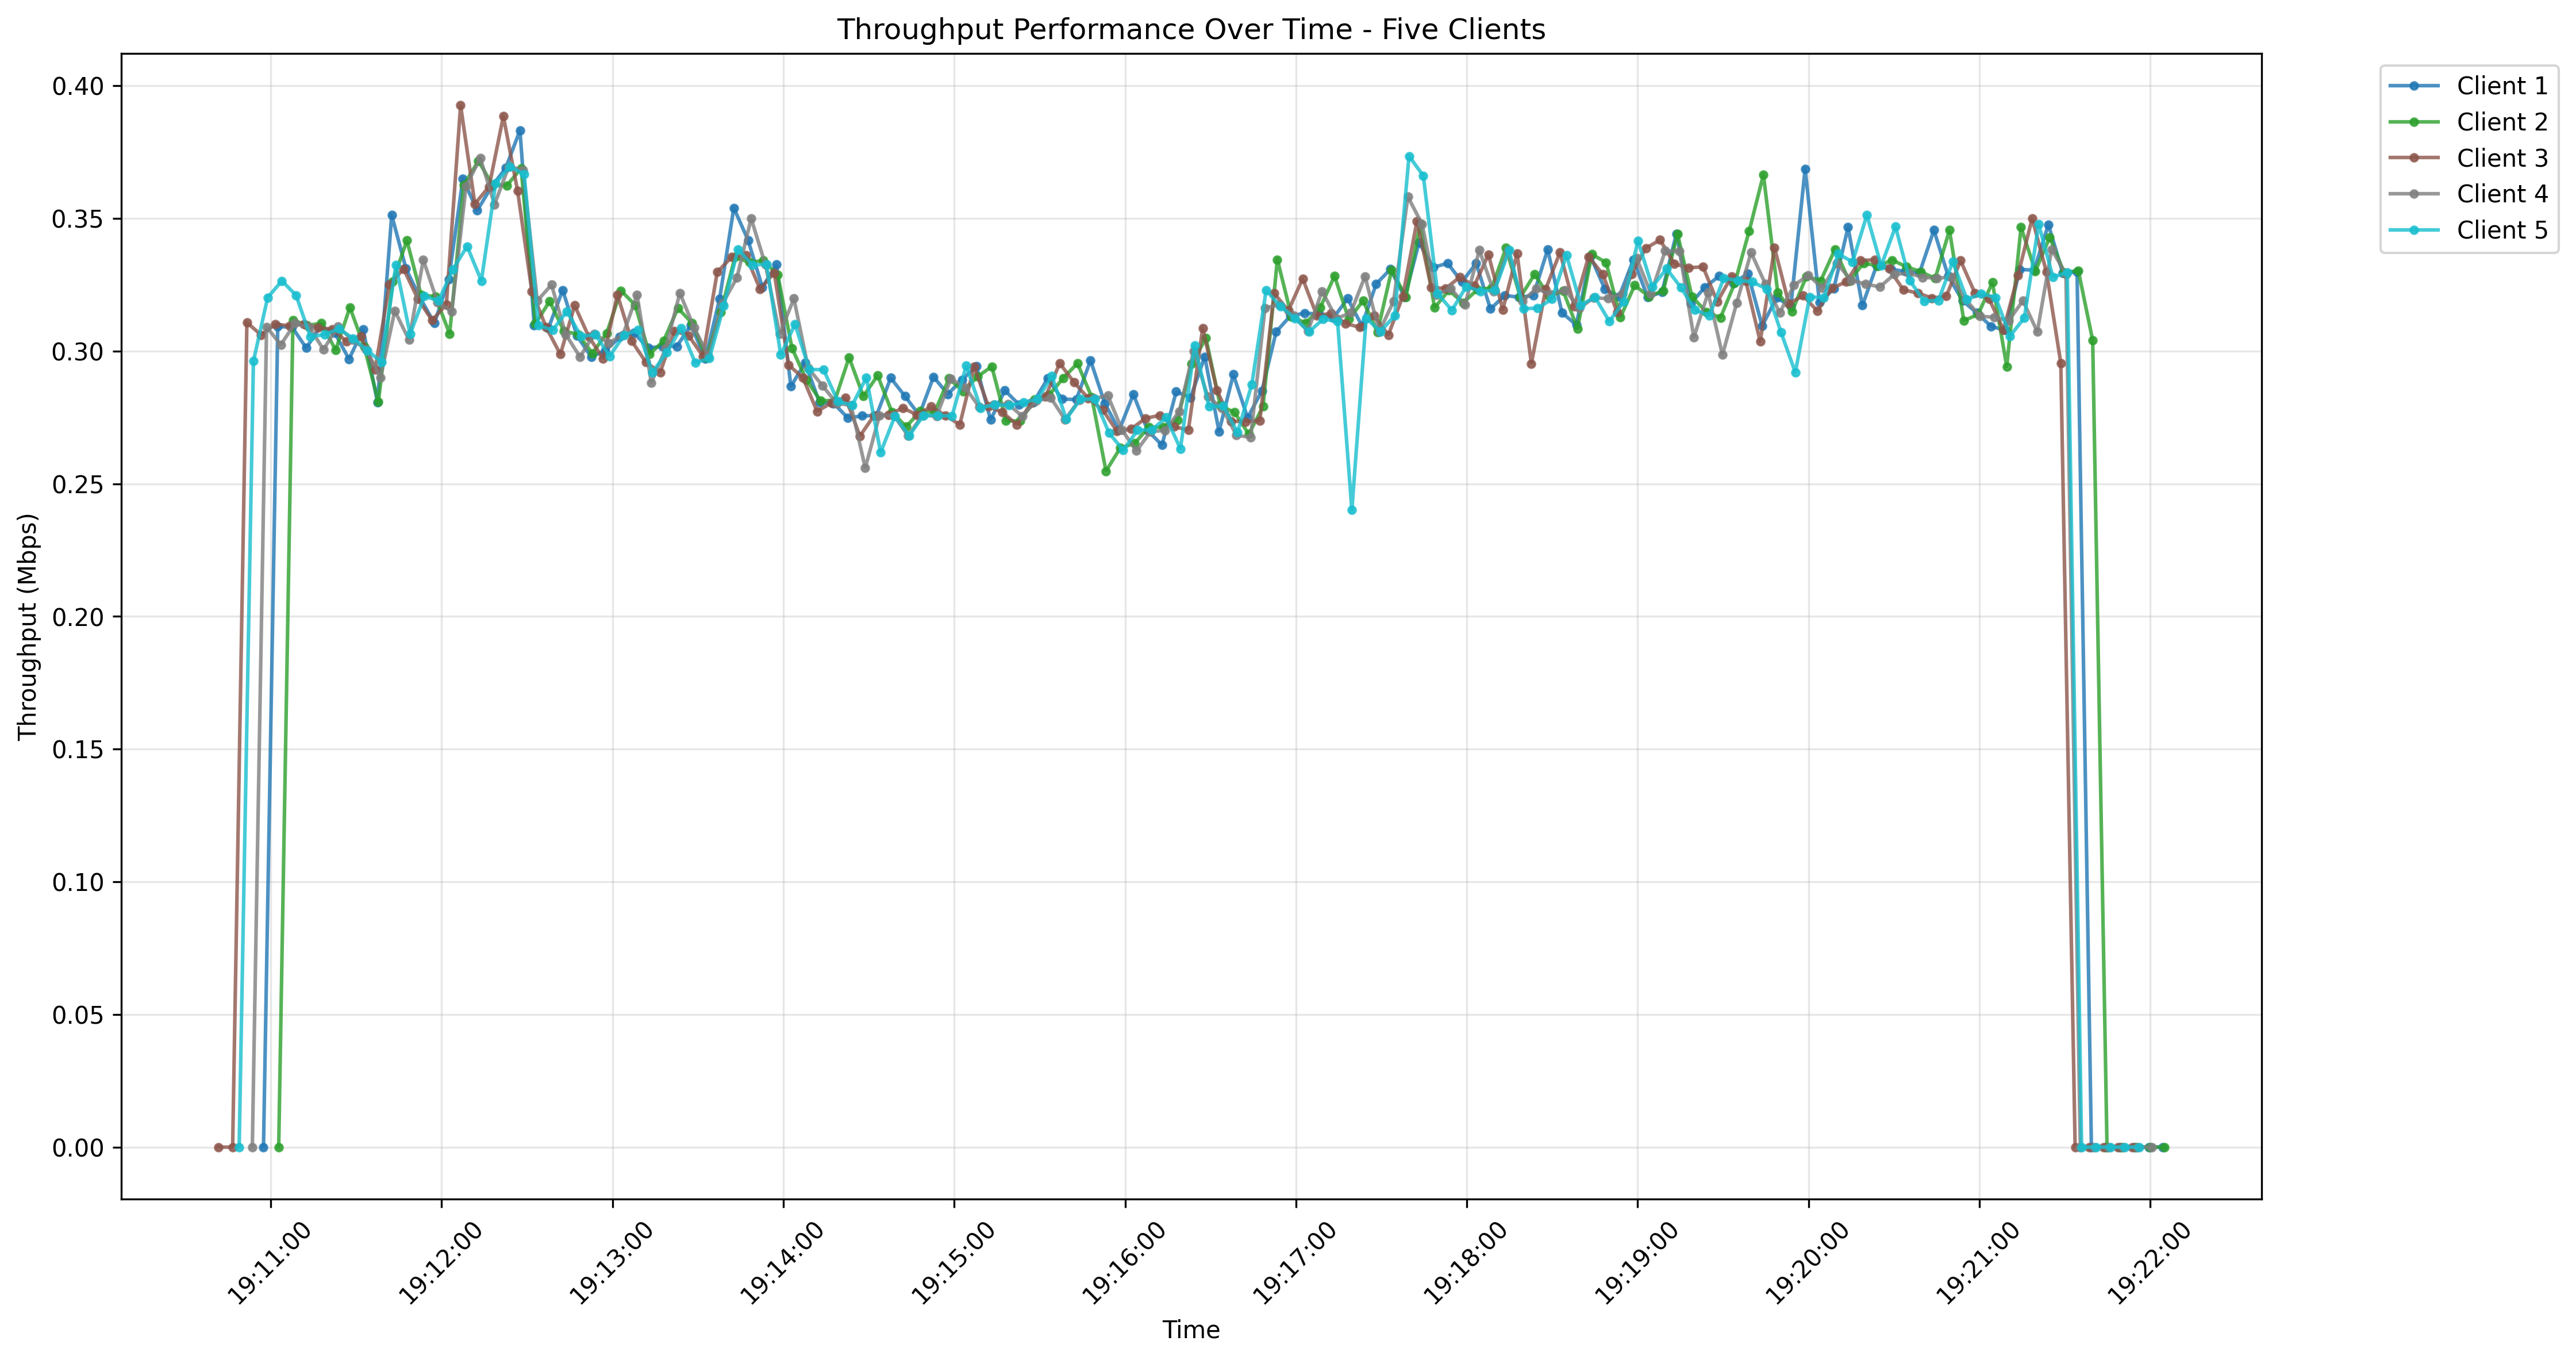
\includegraphics[width=0.8\textwidth]{Evaluation/throughput_by_client_five-clients.png}
\caption{Throughput – Five Clients}
\label{fig:throughput-five-clients}
\end{figure}

Figure~\ref{fig:throughput-five-clients} shows the throughput performance per client, with an average of 0.315 Mbps, an aggregate average of 1.58 Mbps, a peak of 0.395 Mbps, and a lowest trough of 0.23 Mbps. The aggregate trace was smooth, with no multi-second drops until deliberate shutdown.

\begin{figure}[H]
\centering
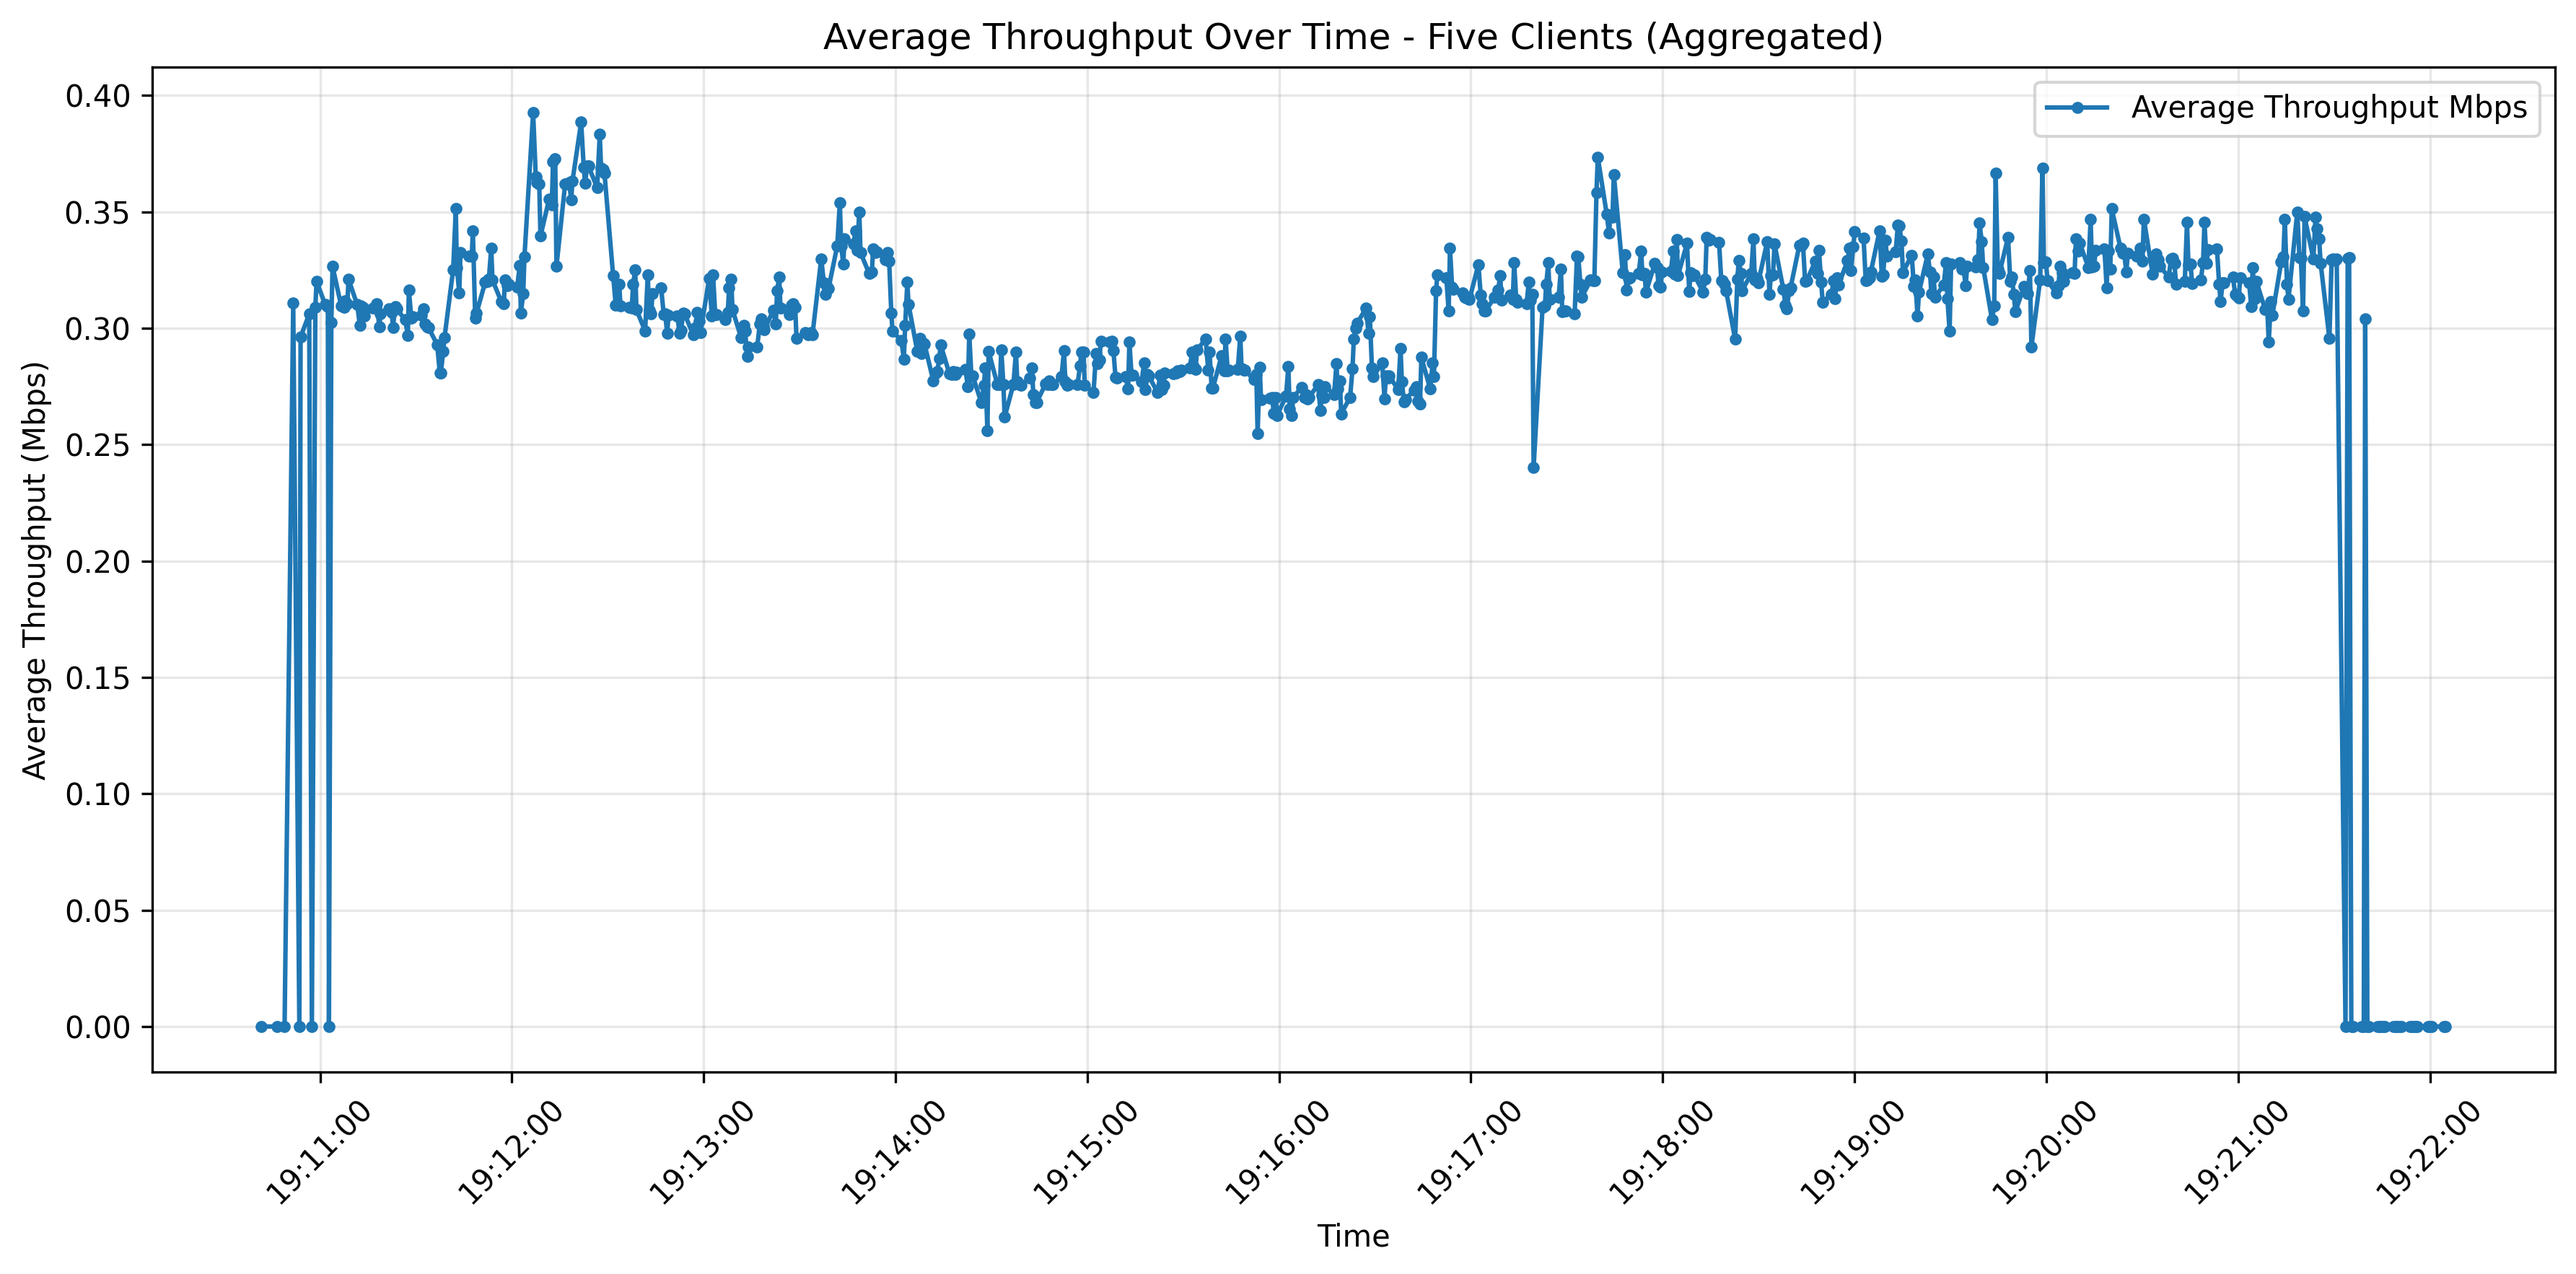
\includegraphics[width=0.8\textwidth]{Evaluation/avg_throughput_aggregated_five-clients.png}
\caption{Aggregated Throughput – Five Clients}
\label{fig:avg-throughput-aggregated-five}
\end{figure}

Figure~\ref{fig:avg-throughput-aggregated-five} presents the combined throughput oscillating between 1.5–1.6 Mbps for most of the run, validating near-linear scaling from the three-client baseline.


\subsubsection{Router Pod Overview}

\begin{figure}[H]
\centering
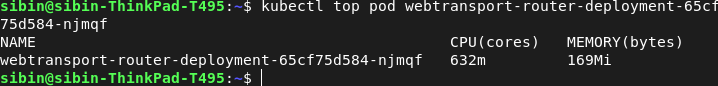
\includegraphics[width=0.8\textwidth]{Evaluation/five-clients-pod-stats.png}
\caption{Router Pod Performance – Five Clients}
\label{fig:router-pod-five-clients}
\end{figure}

Figure~\ref{fig:router-pod-five-clients} shows the router pod performance at 10:54 PM BST on August 5, 2025, utilizing approximately 0.42 core (418 m) of CPU and 92 MiB of memory, with no restarts and stable uptime for 12 minutes. CPU utilisation remained unchanged compared to the three-client run, indicating sub-linear control-plane overhead scaling with client count.

\subsubsection{Host Machine Overview}

\begin{figure}[H]
\centering
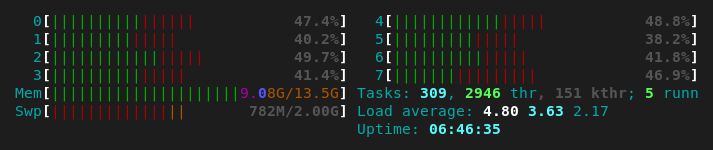
\includegraphics[width=0.8\textwidth]{Evaluation/five-clients-machine-stats.png}
\caption{Host Machine Performance – Five Clients}
\label{fig:host-machine-five-clients}
\end{figure}

Figure~\ref{fig:host-machine-five-clients} depicts the host machine performance at 10:54 PM BST on August 5, 2025, peaking at 40.6\% CPU usage across cores, using 8.53 GiB / 13.5 GiB (63\%) memory, maintaining a load of 2.85 / 2.16 / 2.04, and recording 0 MiB swap usage, comfortably handling the load of additional streams.

\subsubsection{Latency and Processing Time}
Latency remained sub-millisecond, with an average processing time of 0.02–0.03 ms and an average buffer wait time of 0.02–0.03 ms, identical to single- and three-client runs, indicating negligible per-packet overhead.

\subsubsection{Buffer Management}
Buffers auto-tuned from 17 kB to 43 kB, with a peak instantaneous usage of approximately 17 kB per client, and no buffer overflows recorded, demonstrating effective handling of bursty traffic.


\section{System Limitations and Constraints}

\subsection{Identified Limitations}

The system encountered several operational challenges across fragmentation, environment limitations, and protocol-specific constraints. Fragmentation rates consistently exceeded 85\%, primarily due to the 1500-byte MTU restrictions inherent to the Minikube environment. This excessive fragmentation poses a potential risk to throughput performance, especially under sustained load. Environmental constraints, such as Minikube’s limited resource capacity and restricted support for large-scale or multi-node testing, further limited the scope of experimentation. Additionally, protocol-level dependencies introduced complexities, including reliance on a custom packet format, HTTP/3 termination at the proxy, and non-trivial certificate management for local environments. Performance analysis also highlighted bottlenecks under extreme load conditions, particularly in buffer handling, CPU scaling with increased client concurrency, and memory growth driven by the number of active streams. These factors collectively underline the need for robust resource tuning and infrastructure scalability in future deployments.

\section{Validation and Verification}



\subsection{Functional Validation}

The system effectively achieves its core functional objectives. It demonstrates correct stream demultiplexing by accurately separating video, audio, and chat data for independent processing. The protocol translation layer reliably converts incoming HTTP/3 requests to HTTP/1.1, enabling compatibility with downstream microservices. Dynamic routing based on YAML configurations ensures flexibility in directing different stream types to their respective service endpoints. Additionally, integration with Apache Pulsar has been validated through successful message forwarding to the appropriate topics, confirming the system's capability to interface with distributed messaging infrastructure.

\subsection{Performance Validation}

From a performance standpoint, the system meets all key targets. It maintains sub-millisecond processing latency, consistently delivering an average of under 0.1 ms even during peak usage. Throughput remains stable across varying load conditions, indicating robust backpressure handling and internal queuing mechanisms. Resource consumption, both in terms of CPU and memory, remains within acceptable limits, affirming the efficiency of the implementation. Furthermore, scalability tests demonstrate linear performance gains with an increasing number of clients, validating the architecture's suitability for deployment in high-concurrency environments.


\section{Summary}

The comprehensive evaluation confirms that the WebTransport stream routing system meets its design objectives effectively. The router demonstrates reliable handling of multiplexed WebTransport streams while maintaining consistently low latency and stable performance under moderate concurrency. The system achieves a 100\% success rate in packet reconstruction and stream routing, indicating robust processing logic. Throughput and latency metrics remain stable, even as client load increases, and resource consumption is kept within efficient bounds, highlighting sound memory and CPU management. Furthermore, the router integrates seamlessly into the Kubernetes environment, confirming its suitability for cloud-native deployments.

While the current implementation performs reliably, the evaluation also highlights opportunities for future optimization, particularly in reducing fragmentation overhead and supporting larger-scale scenarios. Nonetheless, the findings validate the feasibility and practical value of stream-level routing using WebTransport. The system lays a solid foundation for deploying real-time, low-latency applications within modern, containerized infrastructure.